\section{Análise dos Dados}
\label{sec:analise}

Nesta seção apresentam-se as medições obtidas nos seis ensaios, realizadas com o multímetro digital Victor~88B e o osciloscópio digital Gratten~GA1102CAL, confrontadas com as Eqs.~\eqref{eq:vpico} a~\eqref{eq:ripple} e com as especificações dos componentes. Cada informação é classificada como medida (captura ou leitura), calculada (equação mostrada), de \textit{datasheet} (com citação) ou hipótese (rotulada como \textit{hipótese, não verificada}). Para o osciloscópio, informam-se o valor exibido, o fator aplicado e o valor real. O fator de atenuação $10\times$ (fator $1/10$ sobre o valor exibido) dos Experimentos~1 e~2B foi validado pela plausibilidade dos valores e pela leitura de $17{,}96\,\text{V}$ no multímetro; para a amplitude do \textit{ripple} (Experimentos~3 e~4), o fator da ponta não foi registrado e não está validado.

\subsection{Experimento 1 --- Saída do Transformador (Pré-Retificação)}

\textbf{Condição:} secundário em vazio, com a derivação central (fio preto) como referência de $0\,\text{V}$, antes dos diodos. As Figuras~\ref{fig:exp1-proto}, \ref{fig:exp1-multi} e~\ref{fig:exp1-osc} mostram, respectivamente, a montagem, a leitura do multímetro e a captura do osciloscópio.

\begin{figure}[H]
\centering
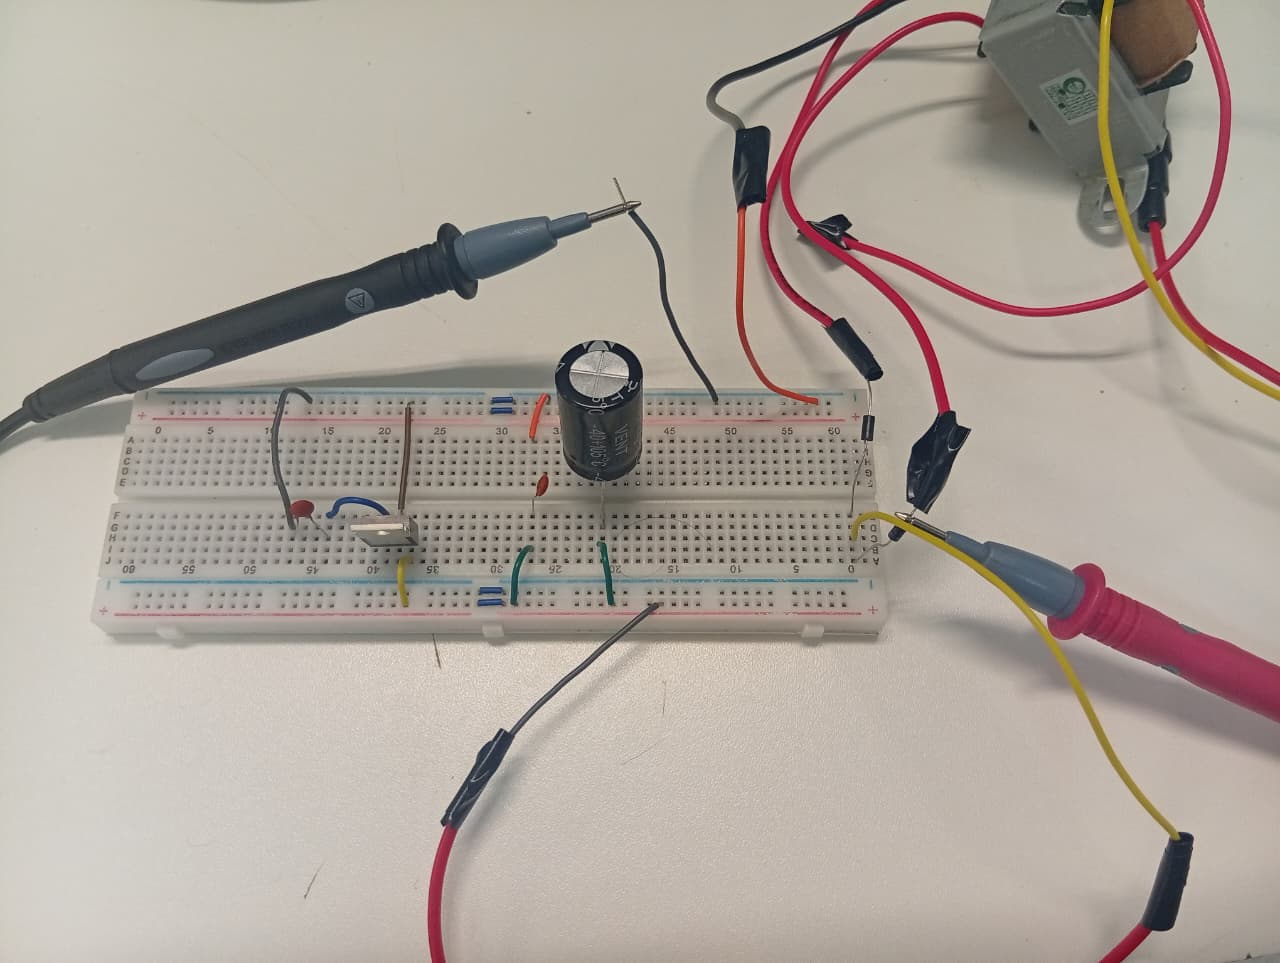
\includegraphics[width=\columnwidth,height=5.6cm,keepaspectratio]{Images/exp1_protoboard-multimetro.jpeg}
\caption{Experimento 1 --- Montagem para medição no secundário do transformador, antes dos diodos.}
\label{fig:exp1-proto}
\end{figure}

\begin{figure}[H]
\centering
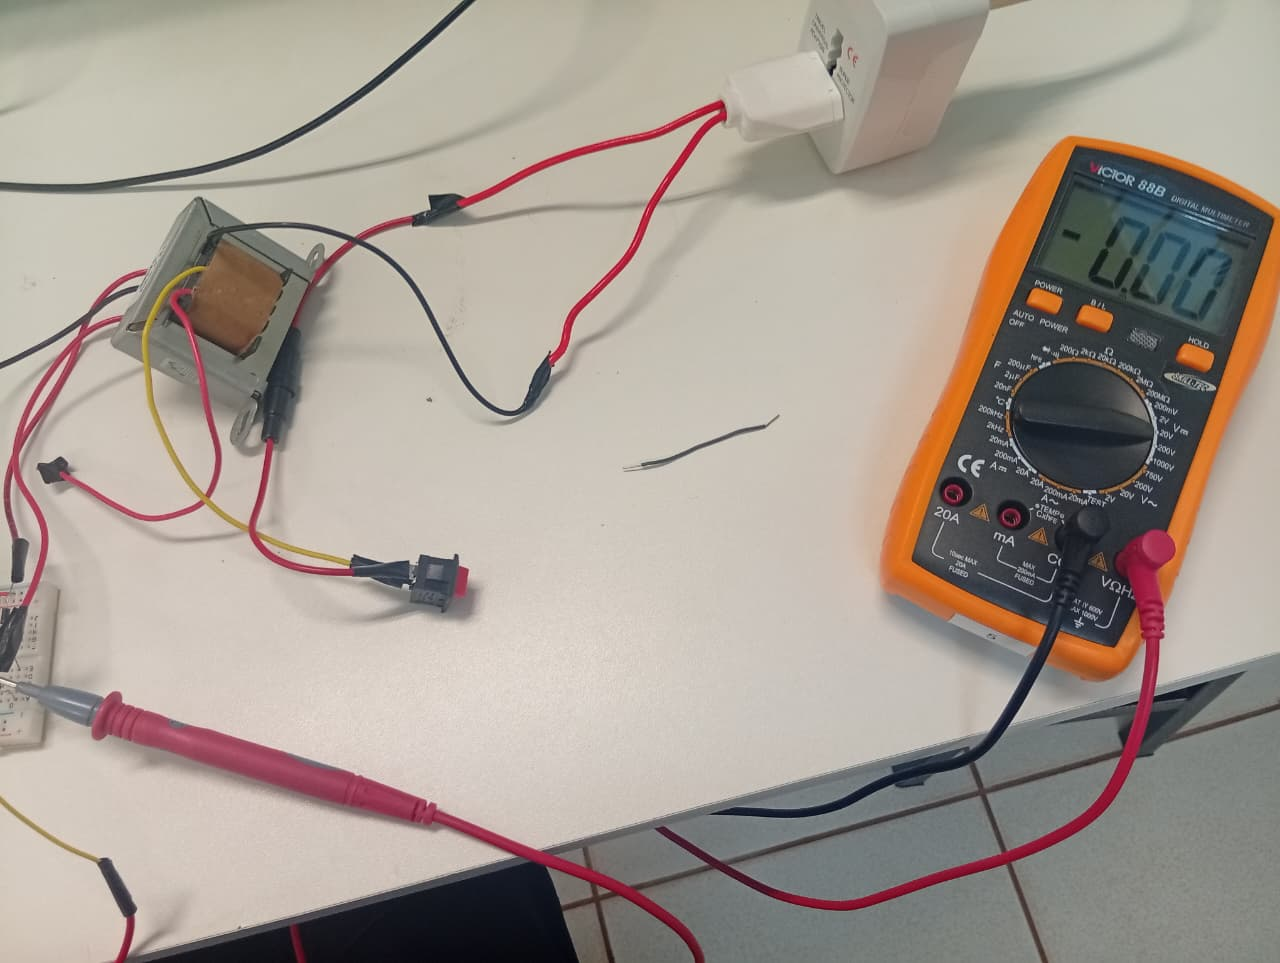
\includegraphics[width=\columnwidth,height=5.6cm,keepaspectratio]{Images/exp1_multimetro.jpeg}
\caption{Experimento 1 --- Multímetro Victor 88B com seletor na escala $20\,\text{V}$ DC, indicando $0{,}00\,\text{V}$. A função correta para o ensaio era V$\sim$ (procedimento incorreto).}
\label{fig:exp1-multi}
\end{figure}

\begin{figure}[H]
\centering
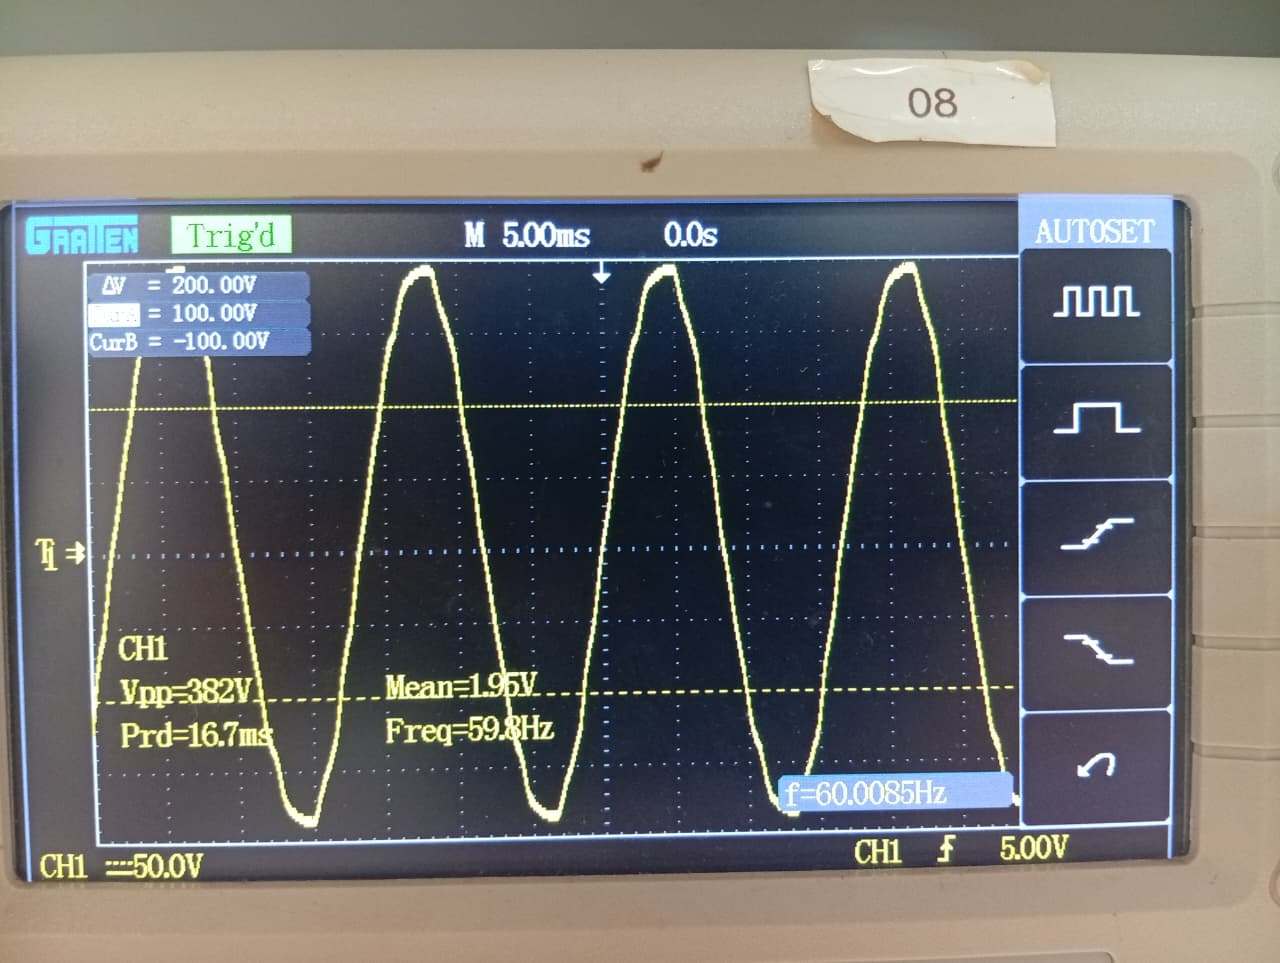
\includegraphics[width=\columnwidth,height=5.6cm,keepaspectratio]{Images/exp1_osciloscopio.jpeg}
\caption{Experimento 1 --- Secundário do transformador ($5{,}00\,\text{ms/div}$, $50{,}0\,\text{V/div}$ exibidos, acoplamento DC, canal em $10\times$ com ponta em $1\times$). Exibido: $V_{\text{pp}} = 382\,\text{V}$; real (fator $1/10$): $38{,}2\,\text{V}$. Contador: $60{,}01\,\text{Hz}$.}
\label{fig:exp1-osc}
\end{figure}

\textbf{Valor exibido e fator.} No osciloscópio (Figura~\ref{fig:exp1-osc}), em modo \textit{Trig'd}, acoplamento DC e \textit{trigger} em $5{,}00\,\text{V}$, o visor indica $V_{\text{pp}} = 382\,\text{V}$ em $50{,}0\,\text{V/div}$, $\text{Mean} = 1{,}95\,\text{V}$, $\text{Prd} = 16{,}7\,\text{ms}$ e $\text{Freq} = 59{,}8\,\text{Hz}$. O canal estava configurado em $10\times$ com a ponta em $1\times$; o valor exibido é, portanto, $10$ vezes o valor real (fator $1/10$). Essa atenuação é coerente com a leitura posterior de $19{,}1\,\text{V}$ de pico no Experimento~2A, obtida com fator $1\times$.

\textbf{Valor real.}
\begin{equation}
V_{\text{pp,real}} = \frac{382\,\text{V}}{10} = 38{,}2\,\text{V}, \qquad V_{p,\text{real}} = \frac{38{,}2\,\text{V}}{2} = 19{,}1\,\text{V}.
\end{equation}
Pela Eq.~\eqref{eq:vpico}, o valor eficaz em vazio é
\begin{equation}
V_{\text{RMS}} = \frac{19{,}1}{\sqrt{2}} \approx 13{,}5\,\text{V},
\end{equation}
valor obtido do osciloscópio, que supõe forma de onda senoidal. O $\text{Mean}$ exibido de $1{,}95\,\text{V}$ corresponde a $0{,}195\,\text{V}$ reais; a janela de $60\,\text{ms}$ (12 divisões de $5{,}00\,\text{ms}$) equivale a $3{,}6$ períodos, o que pode deixar a média da janela diferente de zero (hipótese, não verificada).

\textbf{Esperado e desvio.} Para $12\,\text{V}$ RMS nominais, $V_{\text{RMS}} = 13{,}5\,\text{V}$ representa $+12{,}5\%$. A especificação do trabalho refere-se à tensão nominal do transformador; o valor em vazio é maior que o nominal. Não foi verificado o valor sob carga. A frequência medida no osciloscópio ($59{,}8\,\text{Hz}$, desvio de $-0{,}33\%$ em relação a $60\,\text{Hz}$) tem resolução limitada pelo período exibido ($0{,}1\,\text{ms}$ em $16{,}7\,\text{ms}$); o contador indica $60{,}01\,\text{Hz}$ ($+0{,}01\%$). Observam-se cristas levemente achatadas na forma de onda; a causa não foi investigada.

\textbf{Multímetro.} Com o seletor em $20\,\text{V}$ DC (Figura~\ref{fig:exp1-multi}), o visor indicou $0{,}00\,\text{V}$. Esse valor decorre de falha de procedimento: a medição de tensão alternada exigia a função V$\sim$. A leitura não é resultado do ensaio, e nenhuma medição AC foi obtida com o multímetro.

\subsection{Experimento 2 --- Onda Pós-Diodos (Sem e Com Filtro Capacitivo)}

\textbf{Condição.} Na etapa A, o capacitor de $4700\,\mu\text{F}$ foi removido e um resistor de $1\,\text{k}\Omega$ foi conectado do nó pós-fusível ao GND. Na etapa B, o resistor foi retirado e o capacitor foi reinstalado. As Figuras~\ref{fig:exp2-sem-cap-proto} e~\ref{fig:exp2-sem-cap-osc} referem-se à etapa A, e as Figuras~\ref{fig:exp2-com-cap-proto} e~\ref{fig:exp2-com-cap-osc}, à etapa B.

\begin{figure}[H]
\centering
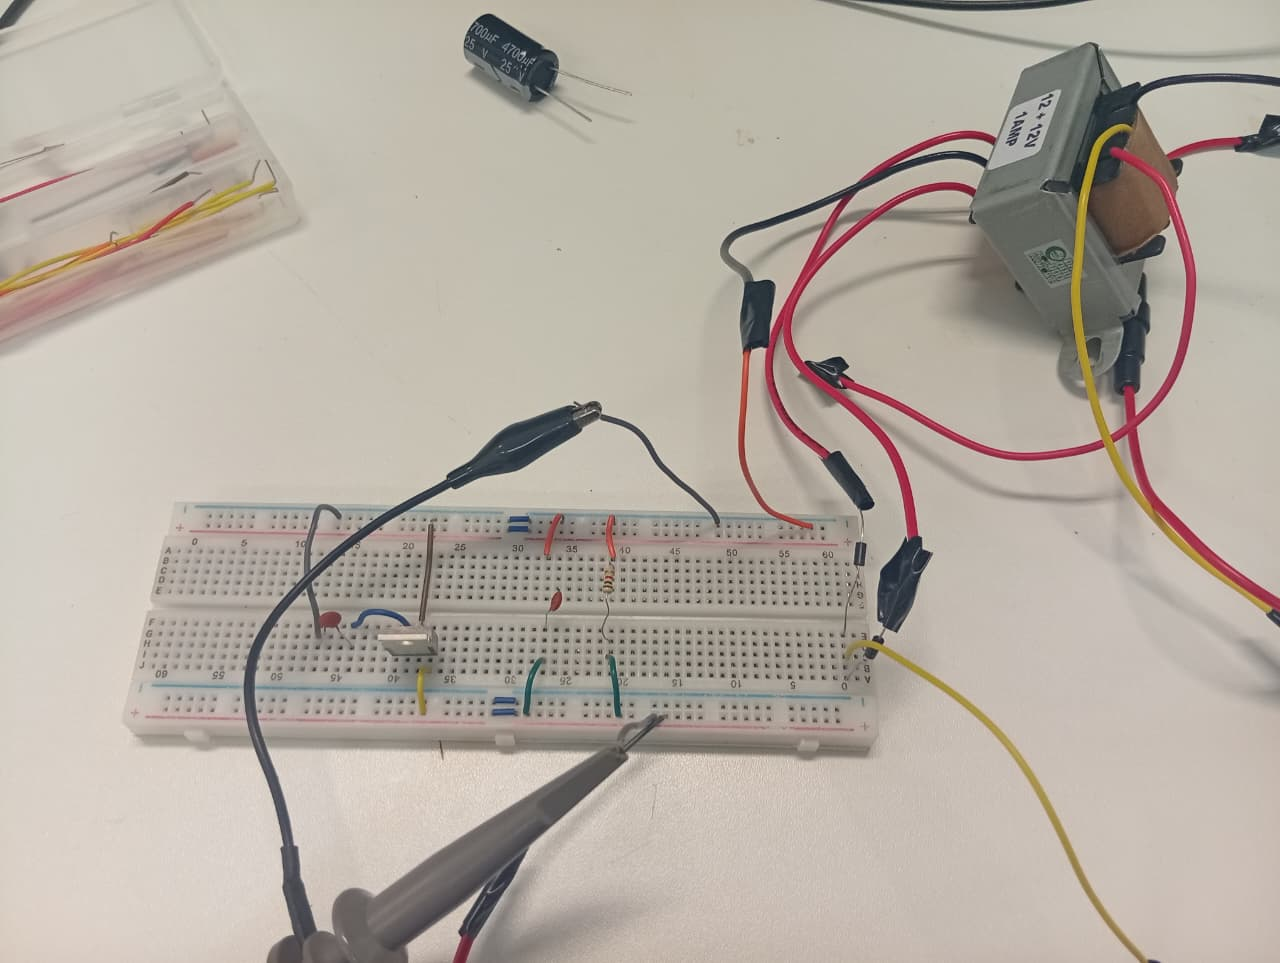
\includegraphics[width=\columnwidth,height=5.6cm,keepaspectratio]{Images/exp2_protoboard-osciloscopio_com-resistencia-1k-ohm.jpeg}
\caption{Experimento 2 (etapa A) --- Montagem sem o capacitor de $4700\,\mu\text{F}$ e com resistor de $1\,\text{k}\Omega$ até o GND.}
\label{fig:exp2-sem-cap-proto}
\end{figure}

\begin{figure}[H]
\centering
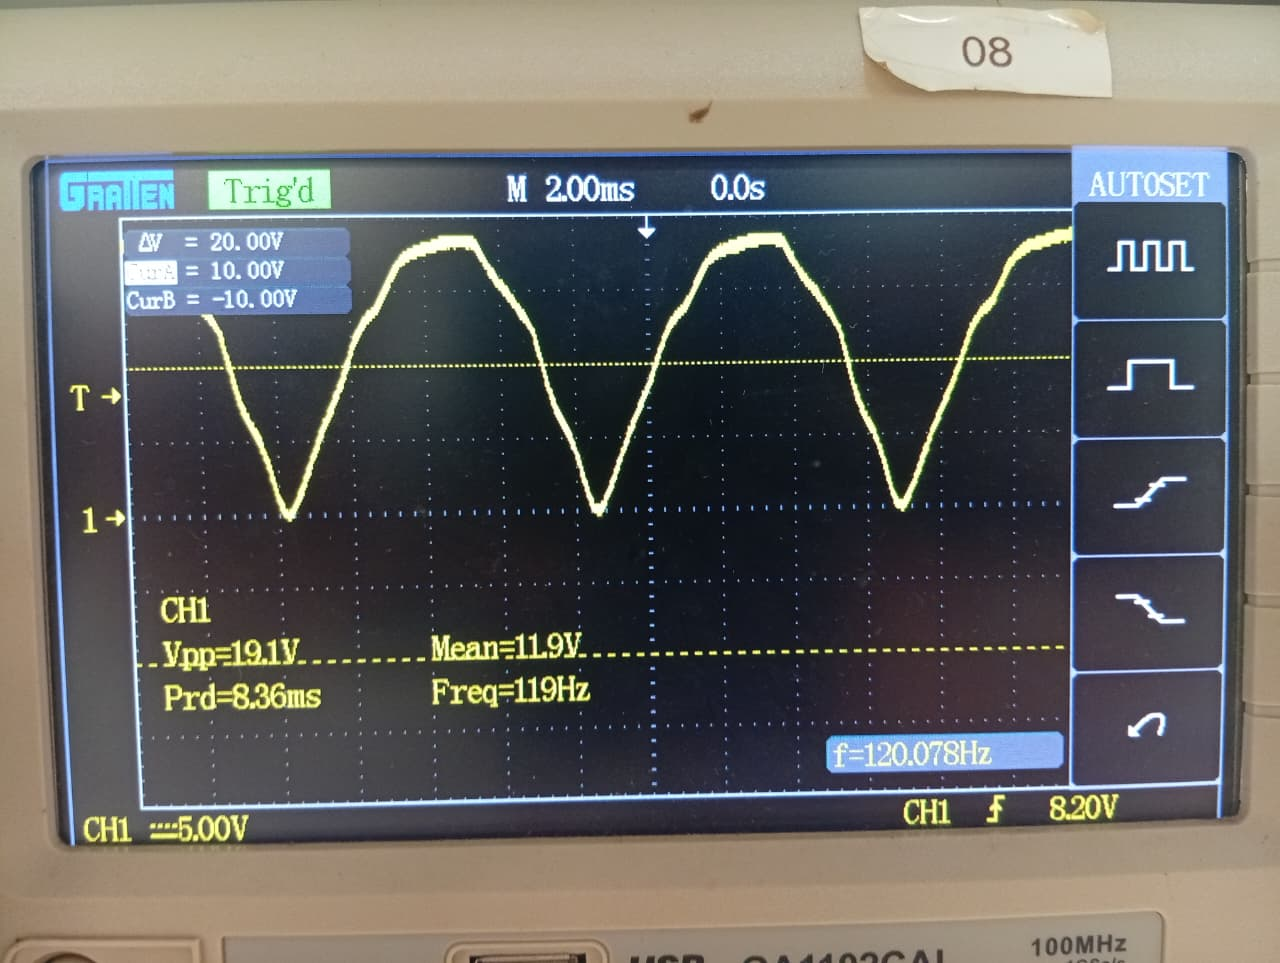
\includegraphics[width=\columnwidth,height=5.6cm,keepaspectratio]{Images/exp2_osciloscopio_com-resistencia-1k-ohm.jpeg}
\caption{Experimento 2 (etapa A) --- Onda retificada sem filtro, acoplamento DC, $5{,}00\,\text{V/div}$, $2{,}00\,\text{ms/div}$, fator $1\times$ (valor real igual ao exibido): $V_{\text{pp}} = 19{,}1\,\text{V}$, $\text{Mean} = 11{,}9\,\text{V}$; contador: $120{,}08\,\text{Hz}$.}
\label{fig:exp2-sem-cap-osc}
\end{figure}

\begin{figure}[H]
\centering
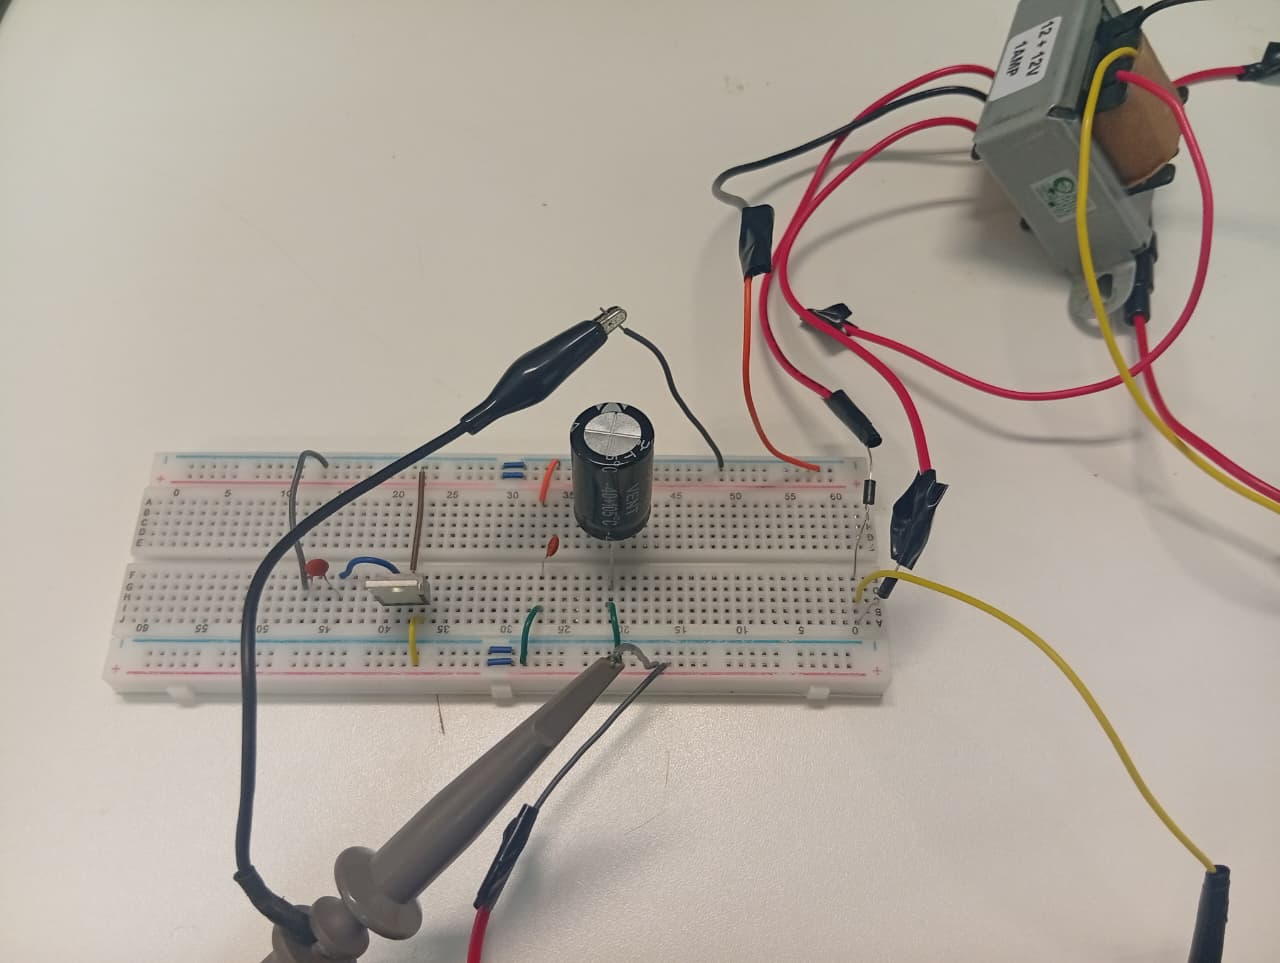
\includegraphics[width=\columnwidth,height=5.6cm,keepaspectratio]{Images/exp2_protoboard-osciloscopio_com-capacitor.jpeg}
\caption{Experimento 2 (etapa B) --- Montagem após a retirada do resistor de $1\,\text{k}\Omega$ e a reinserção do capacitor de $4700\,\mu\text{F}$.}
\label{fig:exp2-com-cap-proto}
\end{figure}

\begin{figure}[H]
\centering
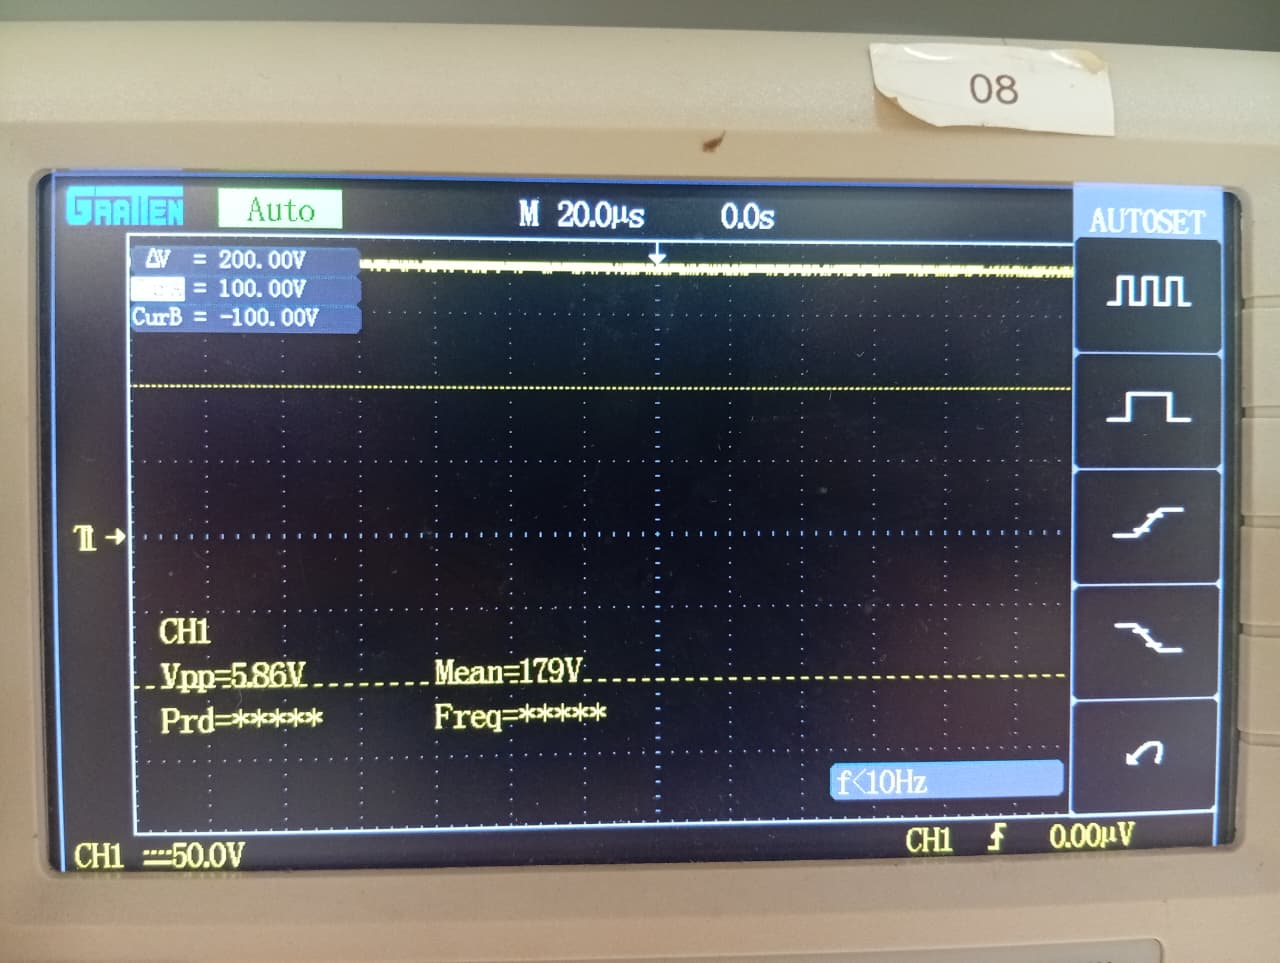
\includegraphics[width=\columnwidth,height=5.6cm,keepaspectratio]{Images/exp2_osciloscopio_com-capacitor.jpeg}
\caption{Experimento 2 (etapa B) --- Captura com filtro capacitivo, acoplamento DC, $50{,}0\,\text{V/div}$ exibidos, $20{,}0\,\mu\text{s/div}$, modo \textit{Auto}, canal em $10\times$ com ponta em $1\times$. Exibido: $\text{Mean} = 179\,\text{V}$; real (fator $1/10$): $\approx 17{,}9\,\text{V}$.}
\label{fig:exp2-com-cap-osc}
\end{figure}

\textbf{Etapa A --- valor exibido, fator e real.} Com $5{,}00\,\text{V/div}$, $2{,}00\,\text{ms/div}$, fator $1\times$ e \textit{trigger} em $8{,}20\,\text{V}$ (Figura~\ref{fig:exp2-sem-cap-osc}), observam-se semiciclos positivos sucessivos a partir da referência de $0\,\text{V}$, o que é compatível com a retificação de onda completa. Os valores exibidos, que coincidem com os reais, são $V_{\text{pp}} = 19{,}1\,\text{V}$, $\text{Mean} = 11{,}9\,\text{V}$, $\text{Prd} = 8{,}36\,\text{ms}$ e $\text{Freq} = 119\,\text{Hz}$; o contador indica $120{,}08\,\text{Hz}$. O período de $8{,}36\,\text{ms}$ difere em $+0{,}3\%$ dos $8{,}33\,\text{ms}$ esperados para $120\,\text{Hz}$.

\textbf{Esperado e desvio.} Com a Eq.~\eqref{eq:vdc_sem_filtro} aplicada a dois valores de pico:
\begin{equation}
V_{\text{DC}} = \frac{2 \times 19{,}1}{\pi} \approx 12{,}16\,\text{V} \quad (V_{p,\text{ret}} = 19{,}1\,\text{V}),
\end{equation}
com desvio $(11{,}9 - 12{,}16)/12{,}16 \approx -2{,}1\%$; e
\begin{equation}
V_{\text{DC}} = \frac{2 \times 18{,}4}{\pi} \approx 11{,}71\,\text{V} \quad (V_{p,\text{ret}} = 19{,}1 - 0{,}7 = 18{,}4\,\text{V}),
\end{equation}
com desvio $(11{,}9 - 11{,}71)/11{,}71 \approx +1{,}6\%$. A média medida concorda com os dois cálculos dentro de $\approx \pm 2\%$, compatível com a resolução de $5\,\text{V/div}$ e com a variação da rede. O desvio não é atribuído à condução dos diodos.

\textbf{Observações sobre os picos.} O pico pós-diodo ($19{,}1\,\text{V}$) é igual ao pico medido antes do diodo no Experimento~1 ($19{,}1\,\text{V}$), embora se espere um valor $\approx 0{,}7\,\text{V}$ menor, isto é, $18{,}4\,\text{V}$. Além disso, os $17{,}96\,\text{V}$ DC com capacitor (Experimento~3) ficam $\approx 1{,}1\,\text{V}$ abaixo de $19{,}1\,\text{V}$ e $\approx 0{,}44\,\text{V}$ abaixo de $18{,}4\,\text{V}$. Como hipótese, não verificada, essas diferenças podem decorrer de variação da rede entre as capturas e da resolução de leitura do osciloscópio; a causa não pôde ser determinada.

\textbf{Etapa B --- valor exibido, fator e real.} Com $50{,}0\,\text{V/div}$, $20{,}0\,\mu\text{s/div}$ e modo \textit{Auto} (Figura~\ref{fig:exp2-com-cap-osc}), o visor indica $\text{Mean} = 179\,\text{V}$ e $V_{\text{pp}} = 5{,}86\,\text{V}$; o contador indica $f < 10\,\text{Hz}$. Com a atenuação $10\times$ (canal em $10\times$ com ponta em $1\times$, fator $1/10$), o valor real é $\text{Mean} \approx 17{,}9\,\text{V}$, diferença de $-0{,}06\,\text{V}$ ($-0{,}3\%$) em relação aos $17{,}96\,\text{V}$ medidos no multímetro no Experimento~3. O valor de $V_{\text{pp}}$ exibido ($5{,}86\,\text{V}$, ou $0{,}586\,\text{V}$ com o fator $1/10$) não é utilizado como resultado, e sua origem não foi determinada.

A janela temporal corresponde a $20\,\mu\text{s/div} \times 12\ \text{divisões visíveis} = 240\,\mu\text{s}$, cerca de $2{,}9\%$ do período de $8{,}33\,\text{ms}$. Essa base de tempo não permite observar o \textit{ripple} nem medir período ou frequência. O resultado válido desta etapa é o nível DC de $\approx 17{,}9\,\text{V}$, confirmado pelo multímetro.

\subsection{Experimento 3 --- Filtro e \textit{Ripple} antes do LM7812 (Pino 1)}

\textbf{Condição.} Mediram-se a tensão DC e a ondulação no pino~1 do LM7812. As Figuras~\ref{fig:exp3-proto} e~\ref{fig:exp3-multi} referem-se à leitura DC, e as Figuras~\ref{fig:exp3-sem-led-osc} e~\ref{fig:exp3-com-led-osc} mostram o \textit{ripple} em acoplamento AC ($2{,}00\,\text{mV/div}$, $5{,}00\,\text{ms/div}$, limite de banda B e filtro F ativos) sem carga na saída e com LED + $1\,\text{k}\Omega$.

\begin{figure}[H]
\centering
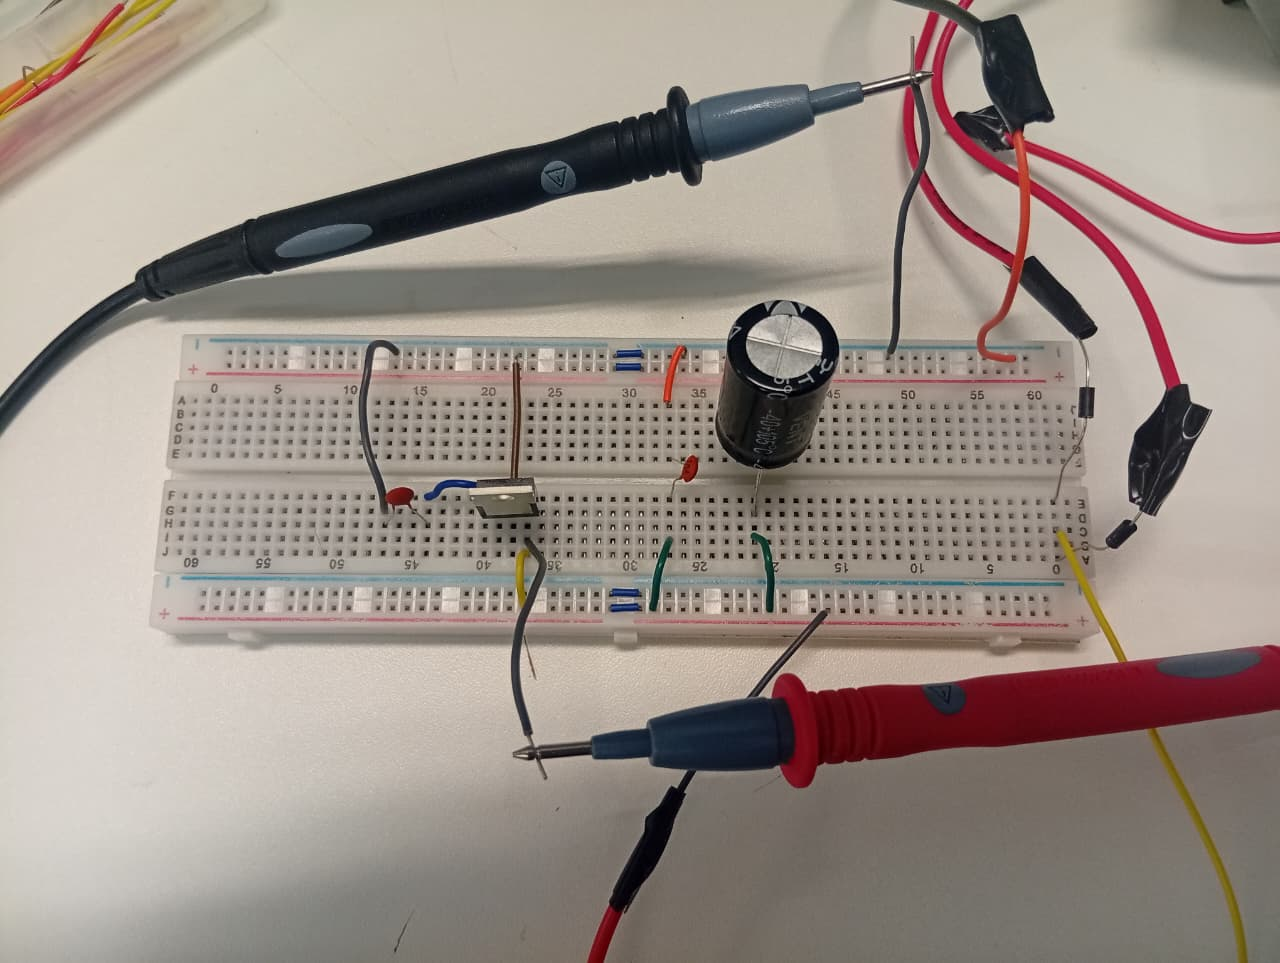
\includegraphics[width=\columnwidth,height=5.6cm,keepaspectratio]{Images/exp3_protoboard-multimetro.jpeg}
\caption{Experimento 3 --- Montagem para medição no pino~1 do LM7812.}
\label{fig:exp3-proto}
\end{figure}

\begin{figure}[H]
\centering
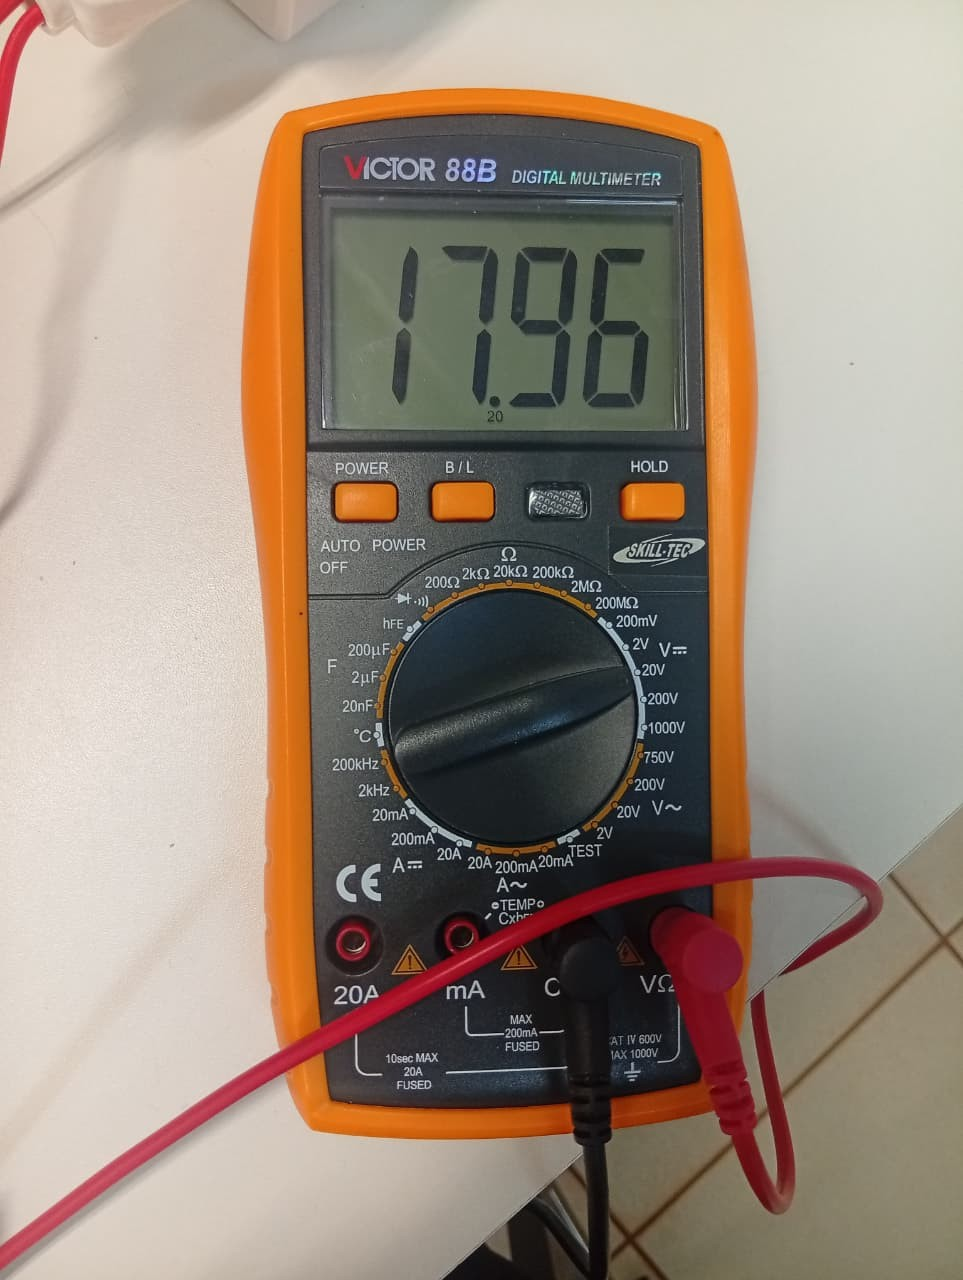
\includegraphics[width=\columnwidth,height=5.6cm,keepaspectratio]{Images/exp3_multimetro.jpeg}
\caption{Experimento 3 --- Multímetro Victor 88B na escala $20\,\text{V}$ DC indicando $17{,}96\,\text{V}$ no pino~1 do LM7812.}
\label{fig:exp3-multi}
\end{figure}

%% Foto de montagem repetida (uma foto de montagem por experimento e mantida na Figura anterior).
%\begin{figure}[H]
%\centering
%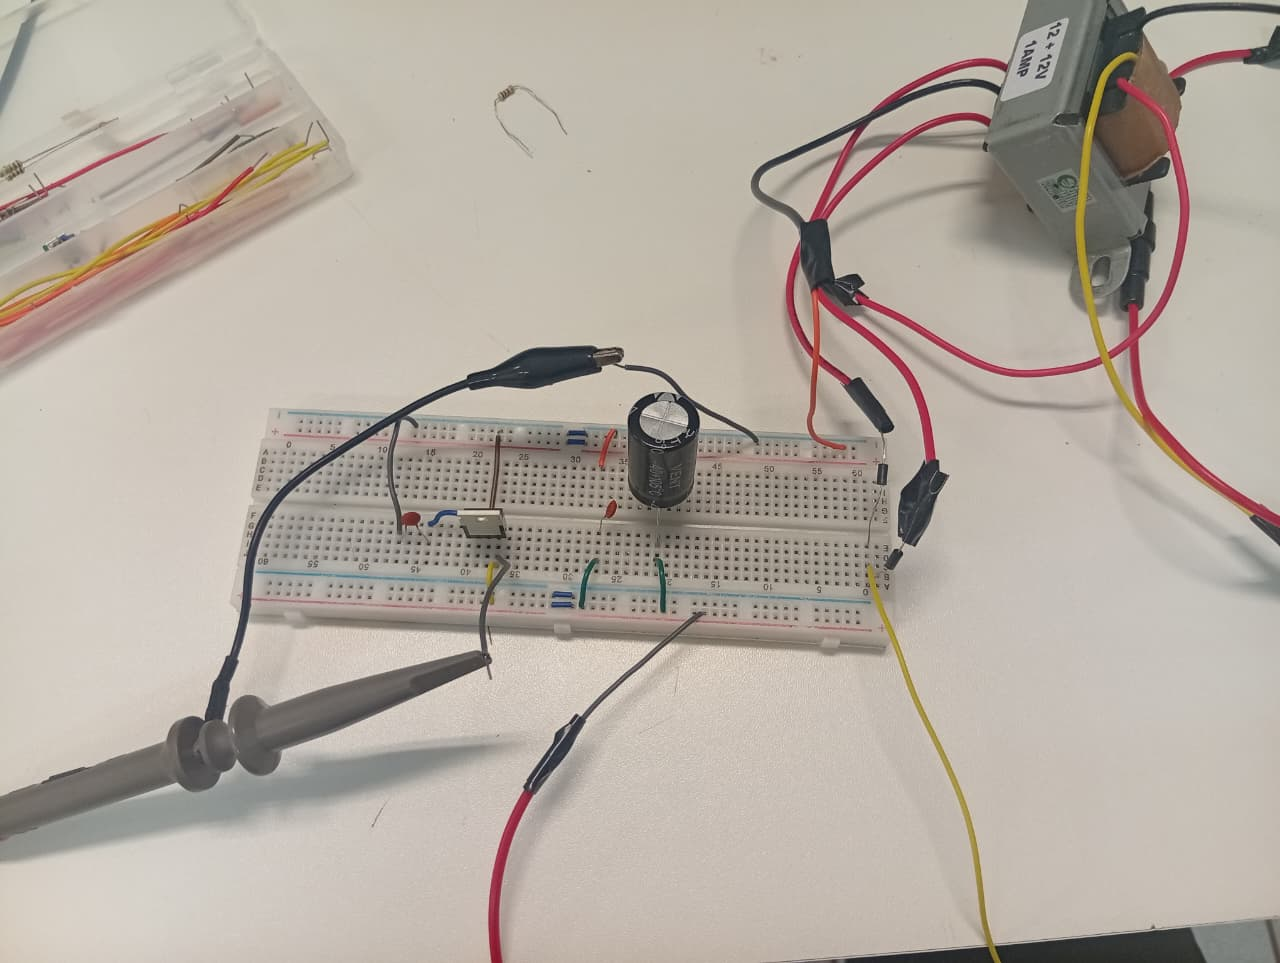
\includegraphics[width=\columnwidth,height=5.6cm,keepaspectratio]{Images/exp3_protoboard-osciloscopio_sem-led-resistencia-1k-ohm.jpeg}
%\caption{Experimento 3 (etapa B) --- Medição no pino~1 do LM7812 sem carga externa na saída de $12\,\text{V}$.}
%\label{fig:exp3-sem-led-proto}
%\end{figure}

\begin{figure}[H]
\centering
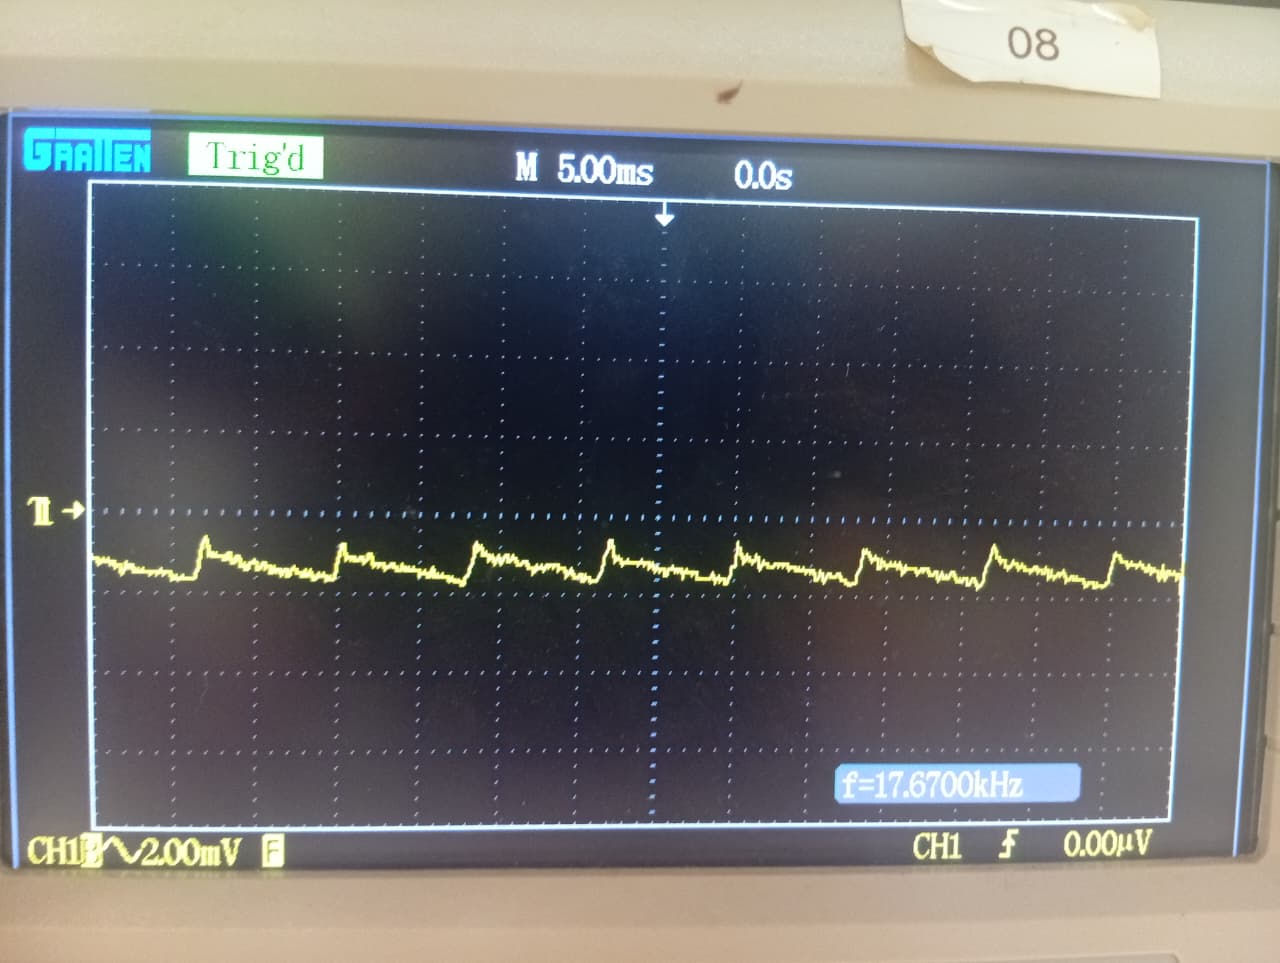
\includegraphics[width=\columnwidth,height=5.6cm,keepaspectratio]{Images/exp3_osciloscopio_sem-led-resistencia-1k-ohm.jpeg}
\caption{Experimento 3 --- Pino~1 sem carga na saída, acoplamento AC, $2{,}00\,\text{mV/div}$ exibidos, $5{,}00\,\text{ms/div}$, B e F ativos, fator da ponta não registrado: dente de serra de $\approx 0{,}6$ a $0{,}7\,\text{div}$, ou $\approx 1{,}2$ a $1{,}4\,\text{mV}_{\text{pp}}$ exibidos.}
\label{fig:exp3-sem-led-osc}
\end{figure}

%% Foto de montagem repetida.
%\begin{figure}[H]
%\centering
%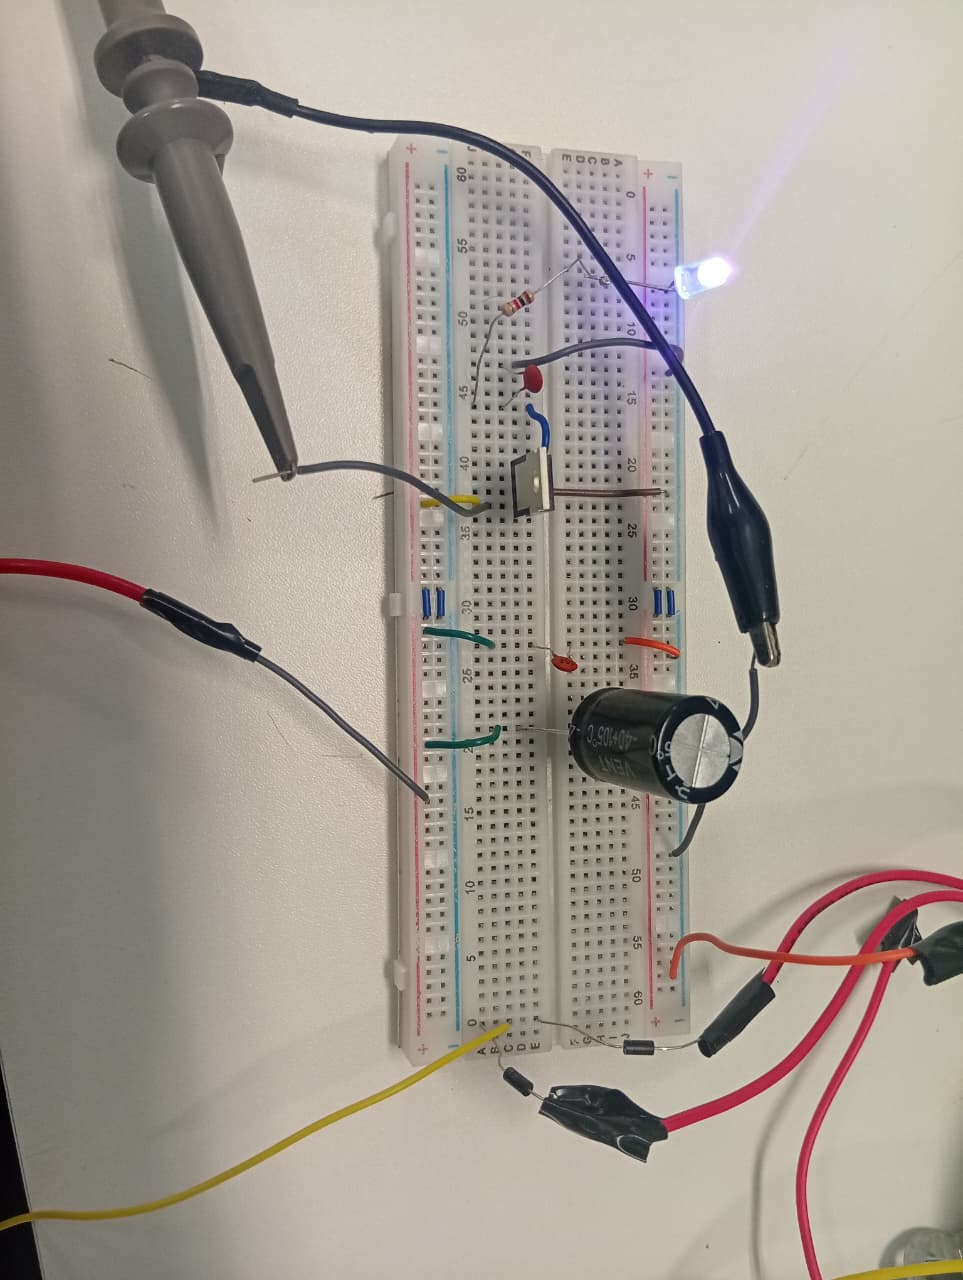
\includegraphics[width=\columnwidth,height=5.6cm,keepaspectratio]{Images/exp3_protoboard-osciloscopio_com-led-resistencia-1k-ohm.jpeg}
%\caption{Experimento 3 (etapa C) --- Medição no pino~1 do LM7812 com LED e resistor de $1\,\text{k}\Omega$ conectados na saída.}
%\label{fig:exp3-com-led-proto}
%\end{figure}

\begin{figure}[H]
\centering
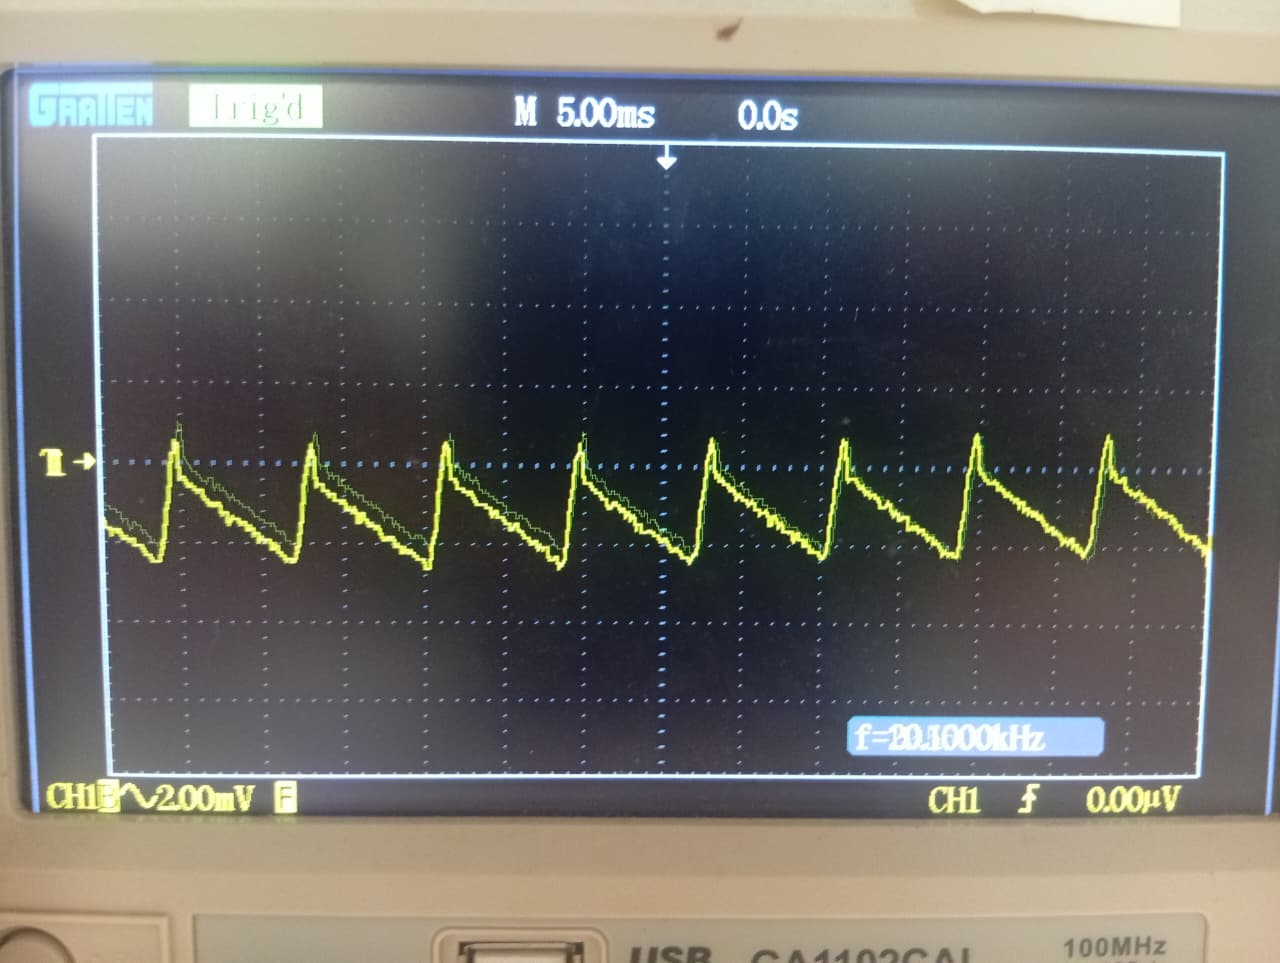
\includegraphics[width=\columnwidth,height=5.6cm,keepaspectratio]{Images/exp3_osciloscopio_com-led-resistencia-1k-ohm.jpeg}
\caption{Experimento 3 --- Pino~1 com LED + $1\,\text{k}\Omega$ na saída, acoplamento AC, $2{,}00\,\text{mV/div}$ exibidos, $5{,}00\,\text{ms/div}$, B e F ativos, fator da ponta não registrado: dente de serra de $\approx 1{,}4$ a $1{,}5\,\text{div}$, ou $\approx 2{,}8$ a $3{,}0\,\text{mV}_{\text{pp}}$ exibidos.}
\label{fig:exp3-com-led-osc}
\end{figure}

\textbf{Validado --- nível DC.} O multímetro (Figura~\ref{fig:exp3-multi}) indicou $17{,}96\,\text{V}$ DC, cerca de $6\,\text{V}$ acima da saída de $12\,\text{V}$ e cerca de $4\,\text{V}$ acima do mínimo de entrada de $14\,\text{V}$ ($12\,\text{V}$ + \textit{dropout} de $\approx 2\,\text{V}$, \textit{datasheet}~\cite{ds_lm7812}). O valor concorda com os $\approx 17{,}9\,\text{V}$ do Experimento~2B.

\textbf{Validado --- forma e crescimento relativo.} Nas Figuras~\ref{fig:exp3-sem-led-osc} e~\ref{fig:exp3-com-led-osc} observa-se forma de dente de serra, com subida rápida e descida gradual, e espaçamento de $\approx 1{,}67\,\text{div} \times 5{,}00\,\text{ms/div} = 8{,}33\,\text{ms}$ entre dentes, compatível com $120\,\text{Hz}$ (cerca de sete a oito dentes na janela de $60\,\text{ms}$). Os valores do contador ($17{,}67\,\text{kHz}$ e $20{,}10\,\text{kHz}$) são artefatos do nível de \textit{trigger} em $0{,}00\,\mu\text{V}$ e não representam a frequência do \textit{ripple}.

Pela Eq.~\eqref{eq:ripple}, com corrente quiescente de $\approx 5\,\text{mA}$ sem carga externa e $\approx 14\,\text{mA}$ com o LED, a razão de correntes é $14/5 = 2{,}8$. A razão das amplitudes lidas é $3{,}0/1{,}3 \approx 2{,}3$. O crescimento relativo com a carga é, portanto, coerente com o previsto. A corrente adicional do LED, $I_L \approx (11{,}95 - 3{,}0)/1000 \approx 9\,\text{mA}$, supõe $V_F \approx 3{,}0\,\text{V}$ (hipótese, não verificada; a tensão sobre o LED não foi medida).

\textbf{Não validado --- amplitude absoluta.} A Eq.~\eqref{eq:ripple} prevê
\begin{equation}
\Delta V_r \approx \frac{5\,\text{mA}}{120 \cdot 4700\,\mu\text{F}} \approx 8{,}9\,\text{mV}_{\text{pp}}
\end{equation}
sem carga externa e
\begin{equation}
\Delta V_r \approx \frac{14\,\text{mA}}{120 \cdot 4700\,\mu\text{F}} \approx 24{,}8\,\text{mV}_{\text{pp}}
\end{equation}
com o LED, contra $\approx 1{,}3$ e $\approx 3{,}0\,\text{mV}_{\text{pp}}$ lidos, isto é, valores lidos $\approx 7$ a $8$ vezes menores ($8{,}9/1{,}3 \approx 6{,}8$ e $24{,}8/3{,}0 \approx 8{,}3$), com desvios de $-85\%$ e $-88\%$. As causas possíveis, todas não verificadas, são: fator da ponta não registrado, filtro F, limite de banda B e valor de corrente quiescente de \textit{datasheet} diferente do real. A comparação quantitativa é inconclusiva, e a amplitude absoluta do \textit{ripple} não é considerada resultado validado.

\subsection{Experimento 4 --- Saída Regulada de $12\,\text{V}$ (Pino 3)}

\textbf{Condição.} Com o LED + $1\,\text{k}\Omega$ conectado na saída, mediram-se a tensão DC e o sinal residual no pino~3 (Figuras~\ref{fig:exp4-proto-multi} a~\ref{fig:exp4-osc}).

\begin{figure}[H]
\centering
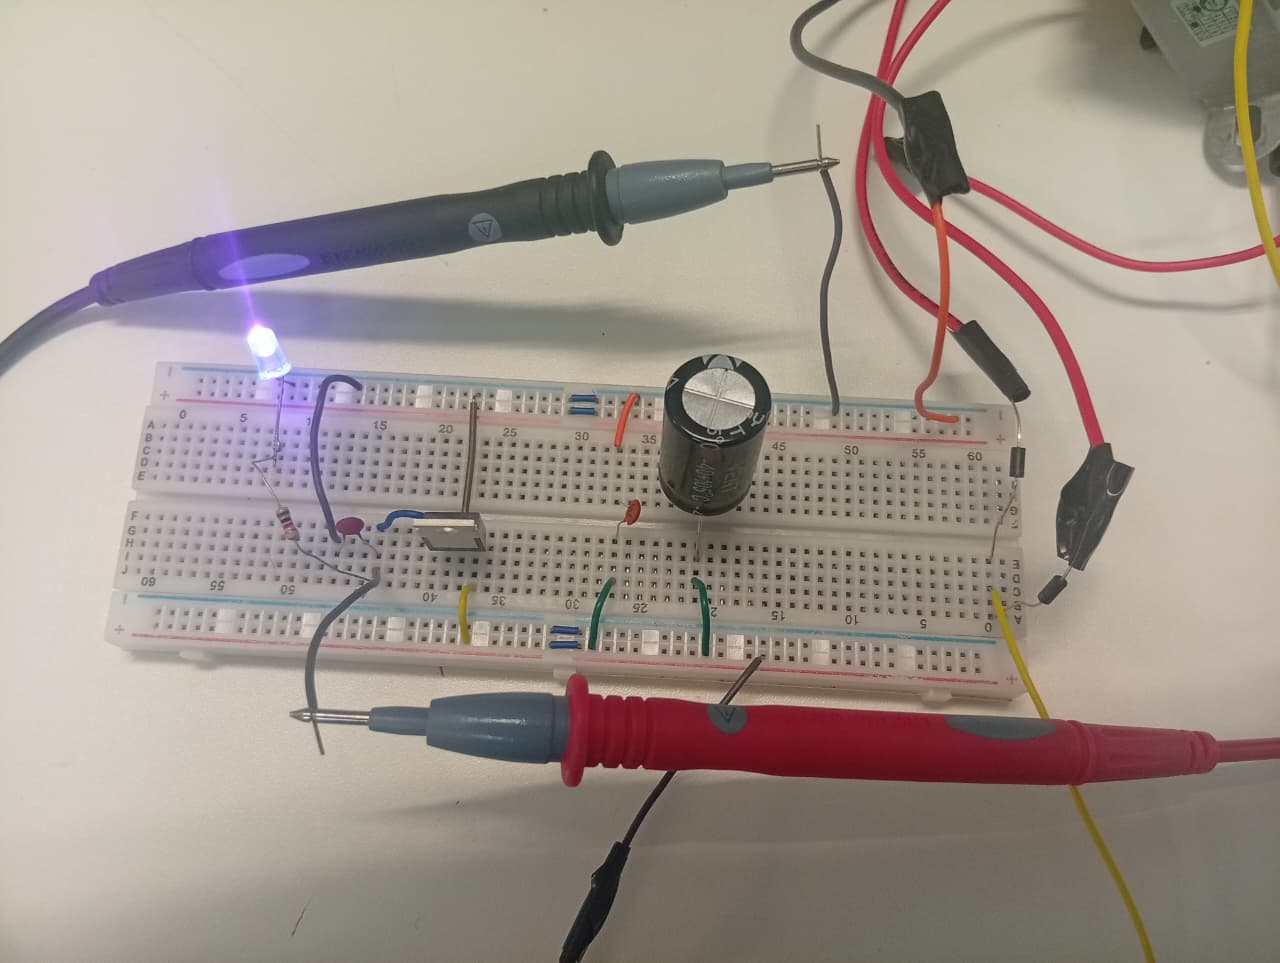
\includegraphics[width=\columnwidth,height=5.6cm,keepaspectratio]{Images/exp4_protoboard-multimetro.jpeg}
\caption{Experimento 4 --- Montagem com a medição no pino~3 do LM7812, com LED e resistor de $1\,\text{k}\Omega$ conectados.}
\label{fig:exp4-proto-multi}
\end{figure}

\begin{figure}[H]
\centering
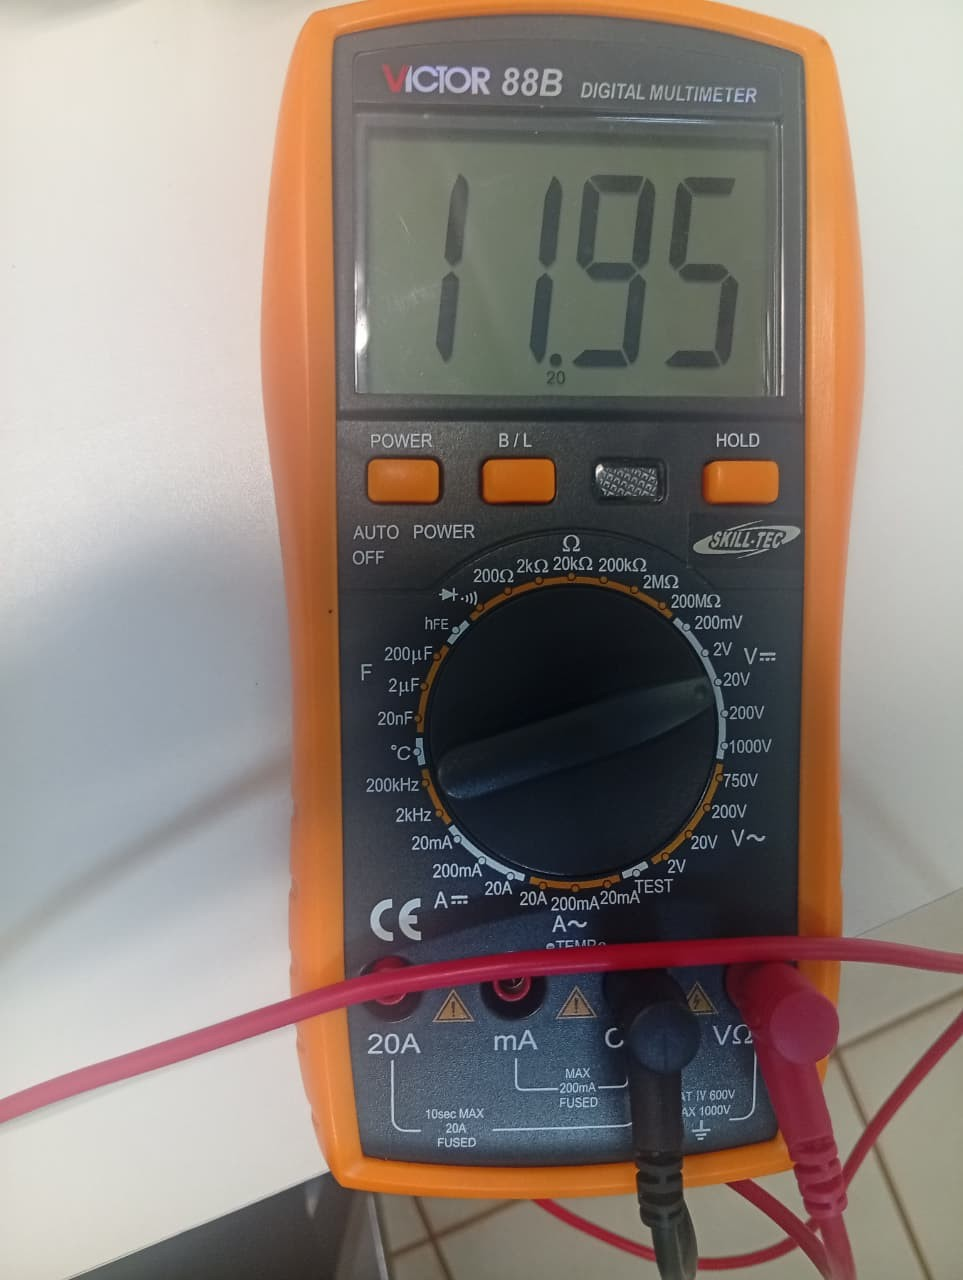
\includegraphics[width=\columnwidth,height=5.6cm,keepaspectratio]{Images/exp4_multimetro.jpeg}
\caption{Experimento 4 --- Multímetro Victor 88B na escala $20\,\text{V}$ DC indicando $11{,}95\,\text{V}$ na saída regulada.}
\label{fig:exp4-multi}
\end{figure}

%% Foto de montagem repetida.
%\begin{figure}[H]
%\centering
%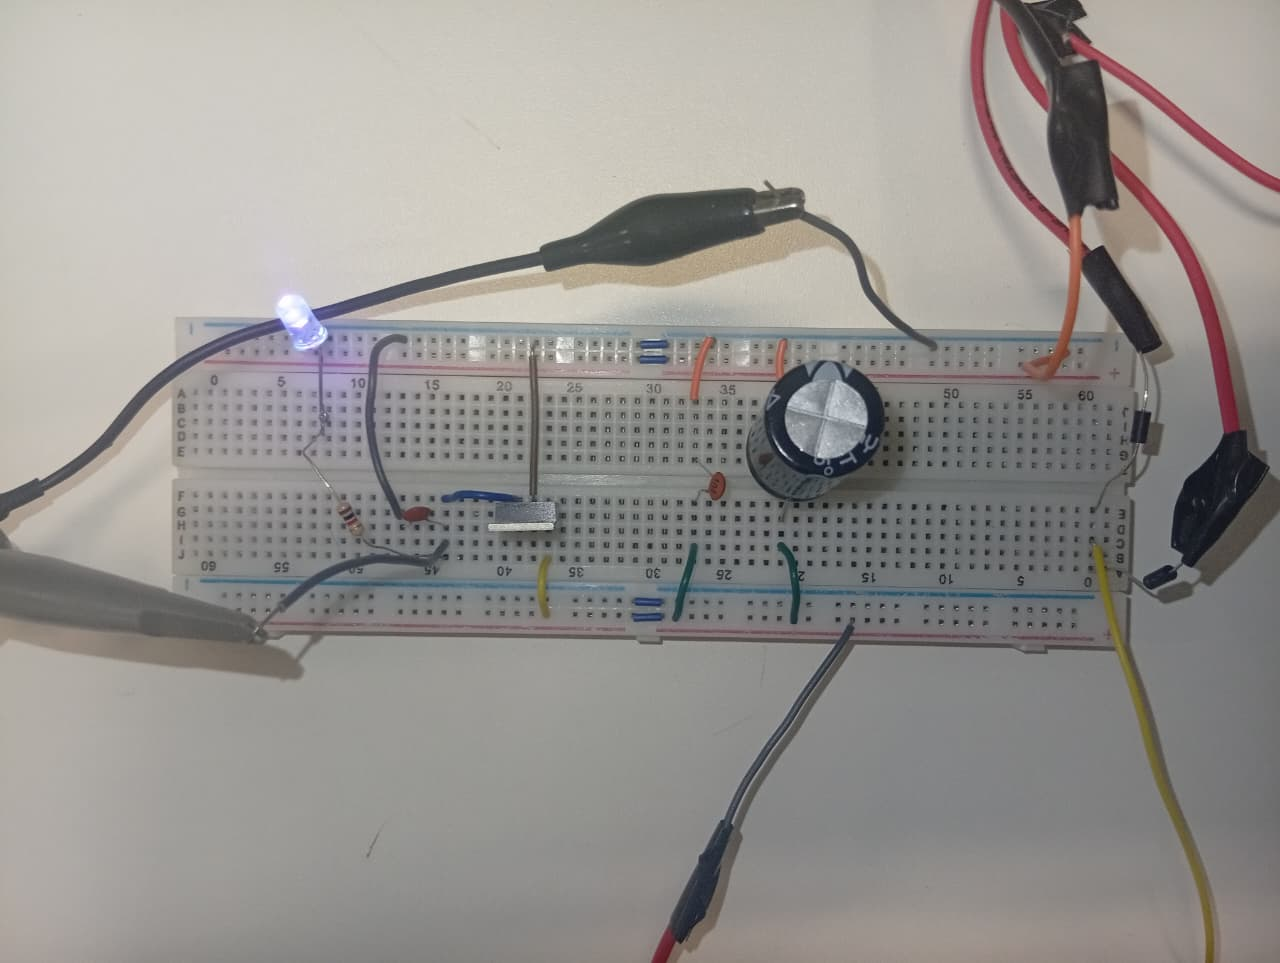
\includegraphics[width=\columnwidth,height=5.6cm,keepaspectratio]{Images/exp4_protoboard-osciloscopio.jpeg}
%\caption{Experimento 4 (etapa B) --- Ponta de prova do osciloscópio no pino~3 do LM7812 com carga ligada.}
%\label{fig:exp4-proto-osc}
%\end{figure}

\begin{figure}[H]
\centering
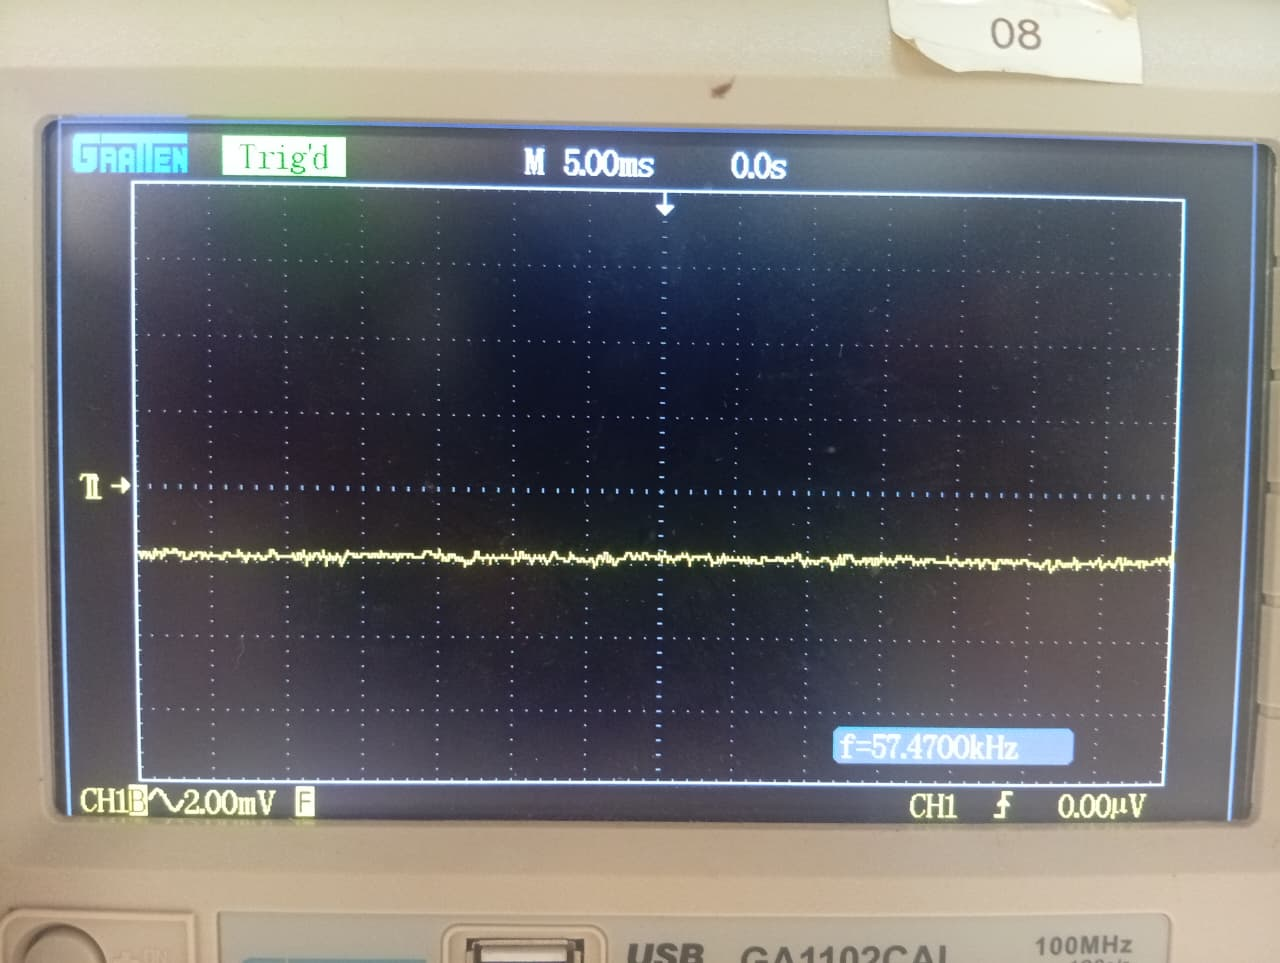
\includegraphics[width=\columnwidth,height=5.6cm,keepaspectratio]{Images/exp4_osciloscopio.jpeg}
\caption{Experimento 4 --- Saída de $12\,\text{V}$ com carga, acoplamento AC, $2{,}00\,\text{mV/div}$ exibidos, $5{,}00\,\text{ms/div}$, B e F ativos, fator da ponta não registrado: traço plano com piso de ruído $\lesssim 0{,}6\,\text{mV}_{\text{pp}}$ exibidos.}
\label{fig:exp4-osc}
\end{figure}

\textbf{Tensão.} O multímetro (Figura~\ref{fig:exp4-multi}) indicou $11{,}95\,\text{V}$ DC. Em relação a $12{,}00\,\text{V}$, o desvio é $(11{,}95 - 12{,}00)/12{,}00 \approx -0{,}42\%$, dentro da faixa de $\pm 4\%$ ($11{,}5\,\text{V}$ a $12{,}5\,\text{V}$, conforme \href{https://www.ti.com/lit/ds/symlink/lm340.pdf}{Datasheet do LM7812}) adotada como critério.

\textbf{\textit{Ripple}.} No osciloscópio (Figura~\ref{fig:exp4-osc}), com a mesma escala vertical, o mesmo acoplamento e a mesma base de tempo do Experimento~3, o traço permanece plano, sem o dente de serra de $120\,\text{Hz}$ do pino~1, com piso de ruído $\lesssim 0{,}6\,\text{mV}_{\text{pp}}$ exibidos. O valor de $57{,}47\,\text{kHz}$ do contador é artefato do \textit{trigger} e não representa sinal na saída. Esse piso é o limite de leitura, e não o valor do \textit{ripple} de saída.

Tomando os valores exibidos nas mesmas configurações, a relação entre a entrada ($\approx 3{,}0\,\text{mV}_{\text{pp}}$) e a saída ($\lesssim 0{,}6\,\text{mV}_{\text{pp}}$) corresponde a uma redução de $\approx 14$ a $16\,\text{dB}$ ($20\log(3{,}0/0{,}6) \approx 14\,\text{dB}$ e $20\log(3{,}0/0{,}5) \approx 15{,}6\,\text{dB}$). Esse valor é apenas um limite inferior, pois o piso de ruído limita a leitura e a configuração da ponta não foi validada. A rejeição de ondulação de $55$ a $70\,\text{dB}$ é valor de \href{https://www.ti.com/lit/ds/symlink/lm340.pdf}{Datasheet do LM7812} e não foi medida neste trabalho.

Os capacitores de $100\,\text{nF}$ não são responsáveis pela rejeição em $120\,\text{Hz}$: nessa frequência, sua reatância é $X_C = 1/(2\pi \cdot 120 \cdot 100\,\text{nF}) \approx 13\,\text{k}\Omega$. Eles servem à estabilidade do regulador e à atenuação de ruído de alta frequência.

\subsection{Experimento 5 --- Teste de Regulação de Carga}

\textbf{Condição.} O multímetro em $20\,\text{V}$ DC foi conectado entre o pino~3 e o GND sem carga (Figuras~\ref{fig:exp5-sem-led-proto} e~\ref{fig:exp5-sem-led-multi}) e com LED + $1\,\text{k}\Omega$ (Figura~\ref{fig:exp5-com-led-multi}).

\begin{figure}[H]
\centering
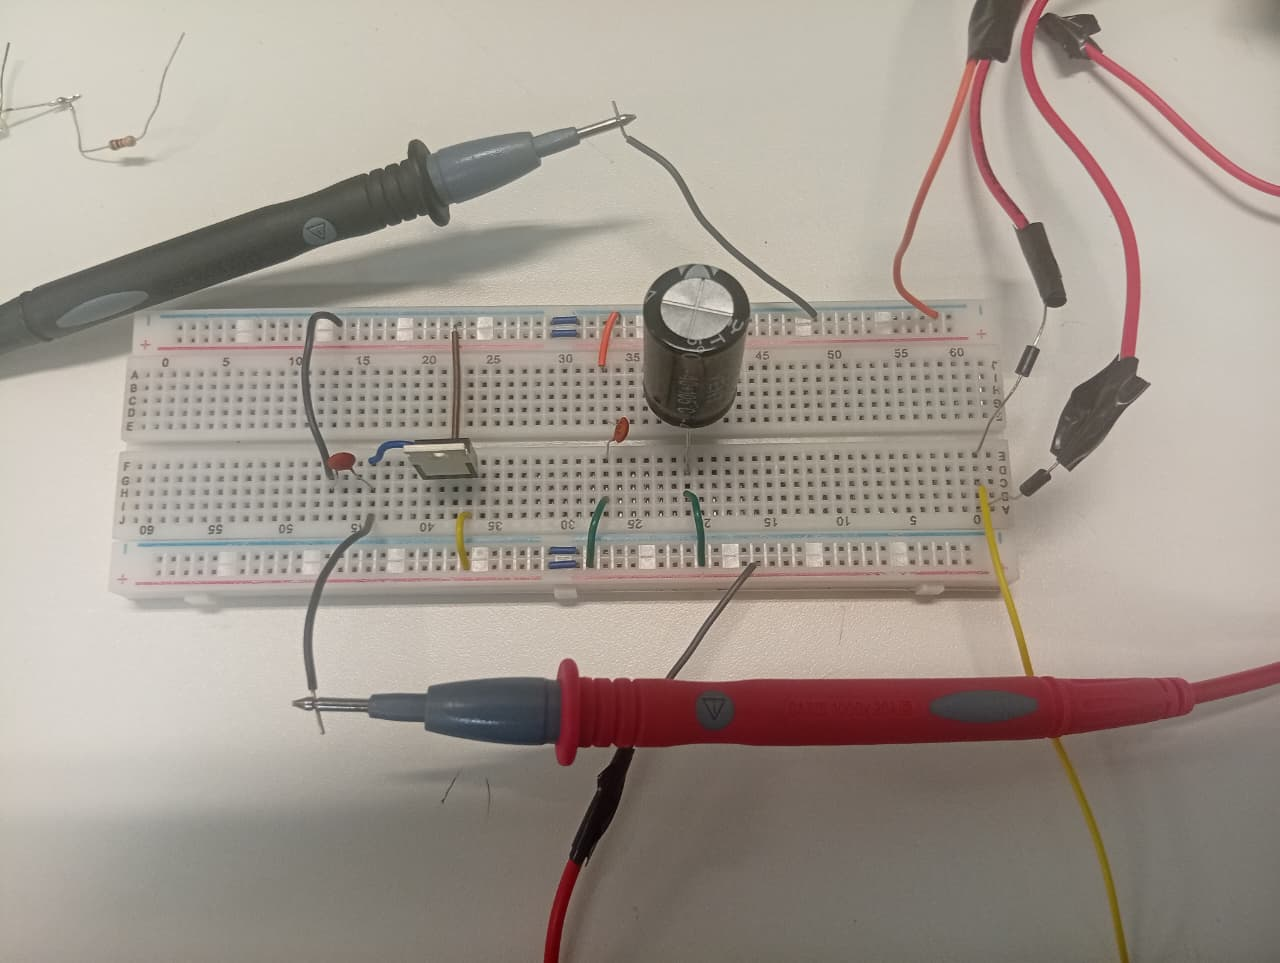
\includegraphics[width=\columnwidth,height=5.6cm,keepaspectratio]{Images/exp5_protoboard-multimetro_sem-led.jpeg}
\caption{Experimento 5 --- Montagem com o multímetro no pino~3, sem carga na saída (LED desconectado).}
\label{fig:exp5-sem-led-proto}
\end{figure}

\begin{figure}[H]
\centering
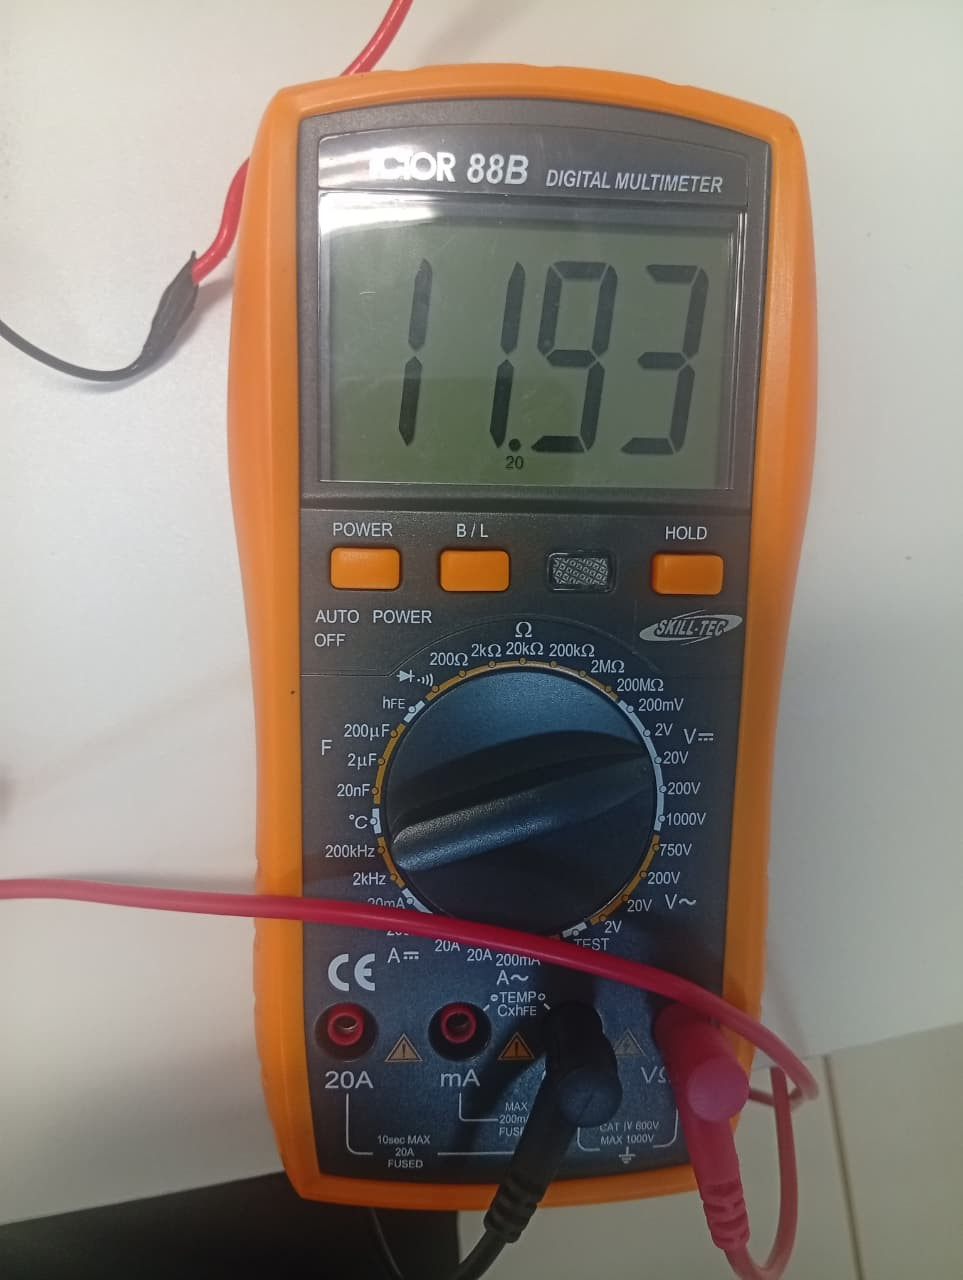
\includegraphics[width=\columnwidth,height=5.6cm,keepaspectratio]{Images/exp5_multimetro_sem-led.jpeg}
\caption{Experimento 5 --- Multímetro Victor 88B na escala $20\,\text{V}$ DC indicando $11{,}93\,\text{V}$ sem carga.}
\label{fig:exp5-sem-led-multi}
\end{figure}

%% Foto de montagem repetida.
%\begin{figure}[H]
%\centering
%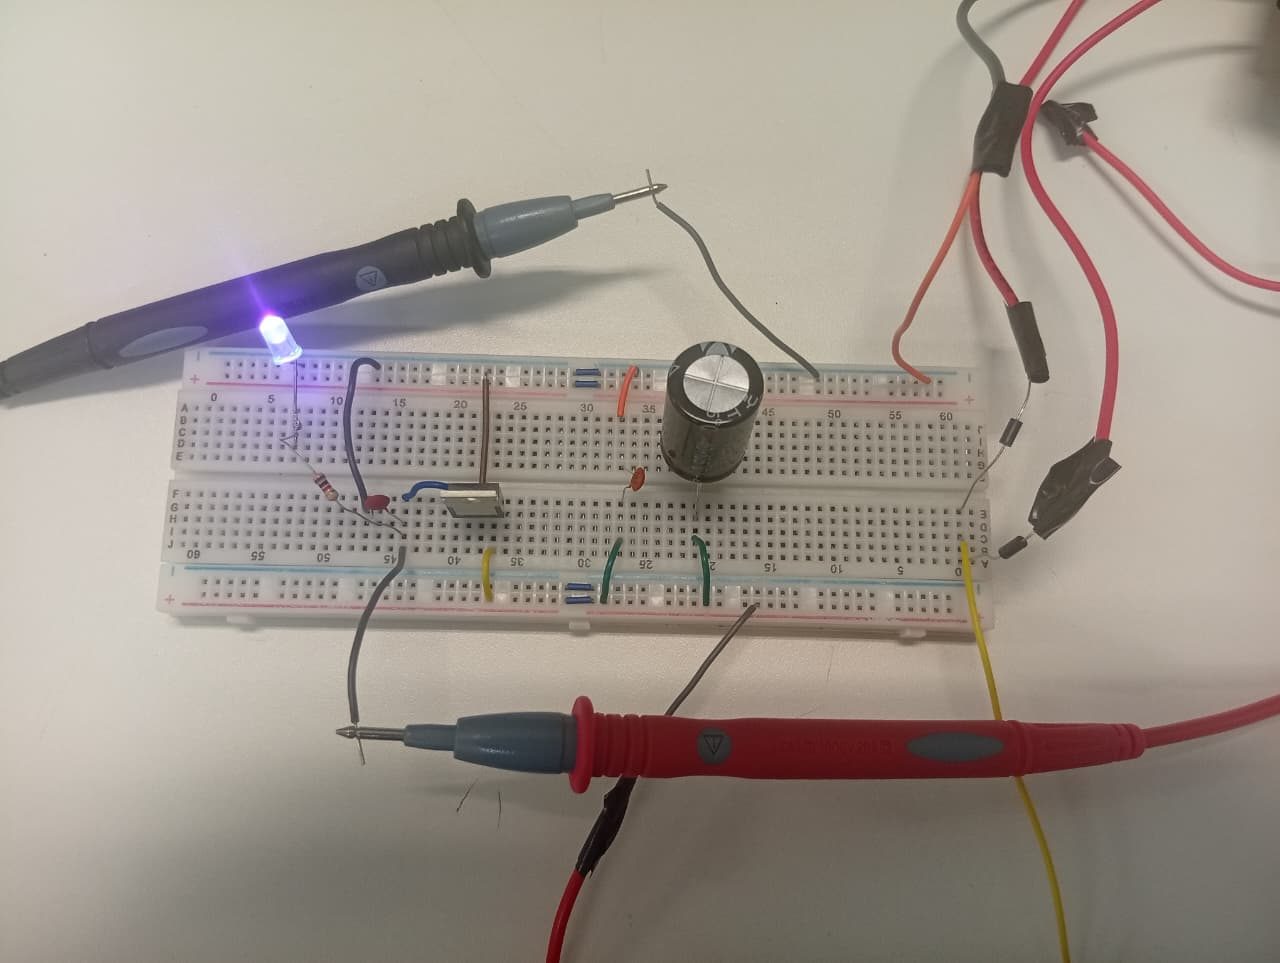
\includegraphics[width=\columnwidth,height=5.6cm,keepaspectratio]{Images/exp5_protoboard-multimetro_com-led.jpeg}
%\caption{Experimento 5 (etapa B) --- Montagem com carga (LED + resistor de $1\,\text{k}\Omega$) conectada.}
%\label{fig:exp5-com-led-proto}
%\end{figure}

\begin{figure}[H]
\centering
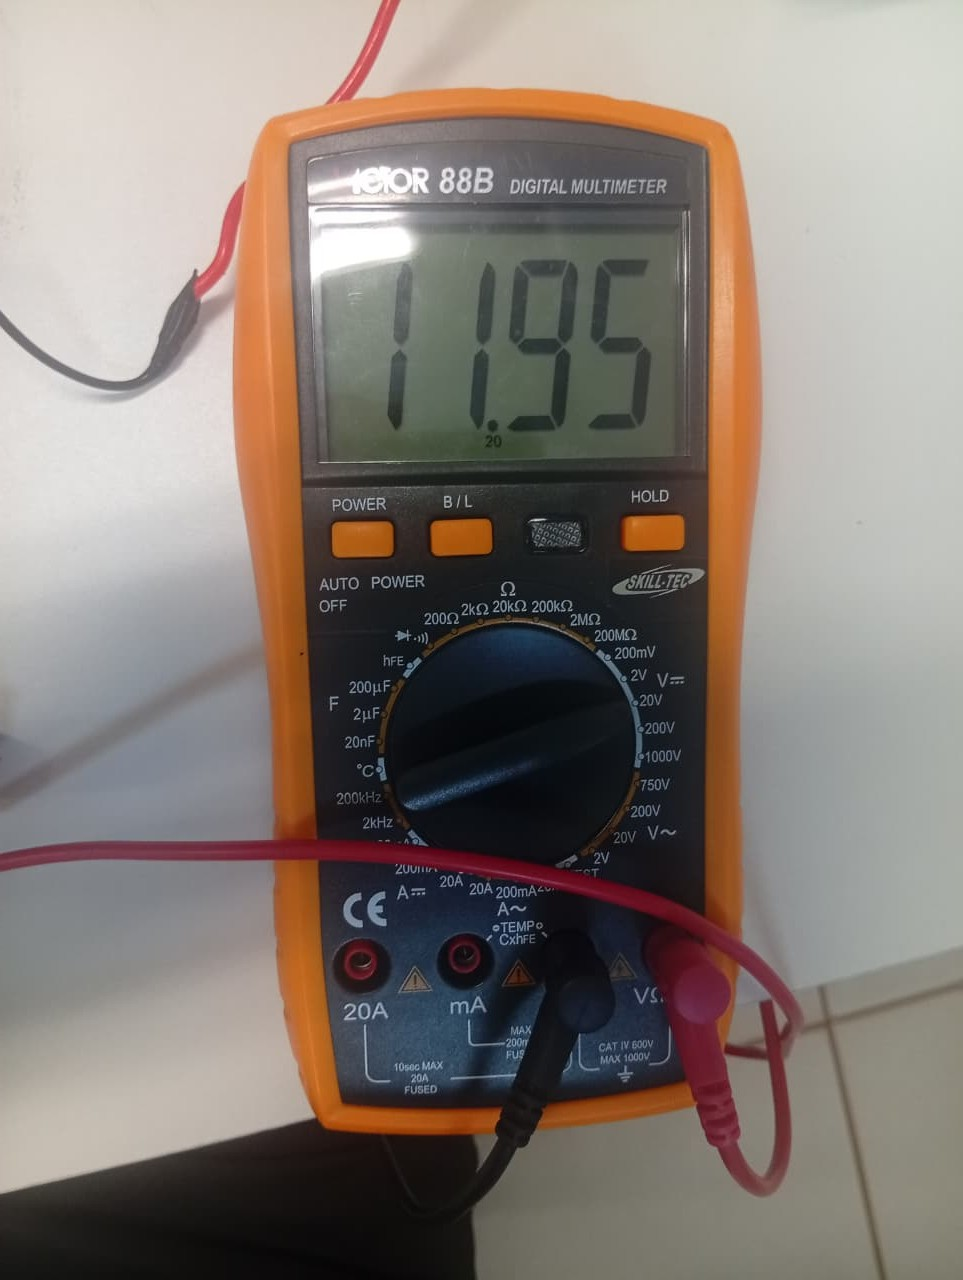
\includegraphics[width=\columnwidth,height=5.6cm,keepaspectratio]{Images/exp5_multimetro_com-led.jpeg}
\caption{Experimento 5 --- Multímetro Victor 88B na escala $20\,\text{V}$ DC indicando $11{,}95\,\text{V}$ com LED + $1\,\text{k}\Omega$.}
\label{fig:exp5-com-led-multi}
\end{figure}

\textbf{Valores medidos.} Sem carga, a leitura foi $11{,}93\,\text{V}$ (Figura~\ref{fig:exp5-sem-led-multi}); com LED + $1\,\text{k}\Omega$, $11{,}95\,\text{V}$ (Figura~\ref{fig:exp5-com-led-multi}), igual à leitura do Experimento~4 na mesma condição. A diferença é $+0{,}02\,\text{V}$.

\textbf{Incerteza e interpretação.} A incerteza adotada para o multímetro na escala de $20\,\text{V}$ DC, $\pm(0{,}5\% + 2\ \text{dígitos})$, resulta em $\pm(0{,}5\% \times 11{,}95 + 0{,}02) \approx \pm 0{,}08\,\text{V}$. As duas leituras são, portanto, indistinguíveis. A tensão não diminuiu com a carga, que seria o sentido esperado, mas aumentou $0{,}02\,\text{V}$, valor inferior à incerteza. A regulação de carga, definida como $(V_{\text{sem}} - V_{\text{com}})/V_{\text{com}}$, é
\begin{equation}
\frac{11{,}93 - 11{,}95}{11{,}95} \approx -0{,}17\%,
\end{equation}
valor menor que a incerteza relativa de $\approx 0{,}67\%$ e sem significado físico próprio. A variação de corrente entre as duas condições, $\Delta I \approx 9\,\text{mA}$ (cálculo com $V_F \approx 3{,}0\,\text{V}$, hipótese, não verificada), não exercita a regulação do LM7812. A tensão sob a carga de $100\,\Omega$ não foi registrada; o valor de $11{,}95\,\text{V}$ usado no Experimento~6 corresponde à condição com LED + $1\,\text{k}\Omega$. Este experimento não tem poder discriminativo para a regulação de carga.

\subsection{Experimento 6 --- Teste de Corrente com Carga de $100\,\Omega$}

\textbf{Condição.} O multímetro foi inserido em série entre o pino~3 do LM7812 e um resistor de $100\,\Omega \pm 5\%$ ligado ao GND, com a ponta vermelha no borne de $20\,\text{A}$ e a ponta preta no borne COM (Figuras~\ref{fig:exp6-proto} e~\ref{fig:exp6-corrente}).

\begin{figure}[H]
\centering
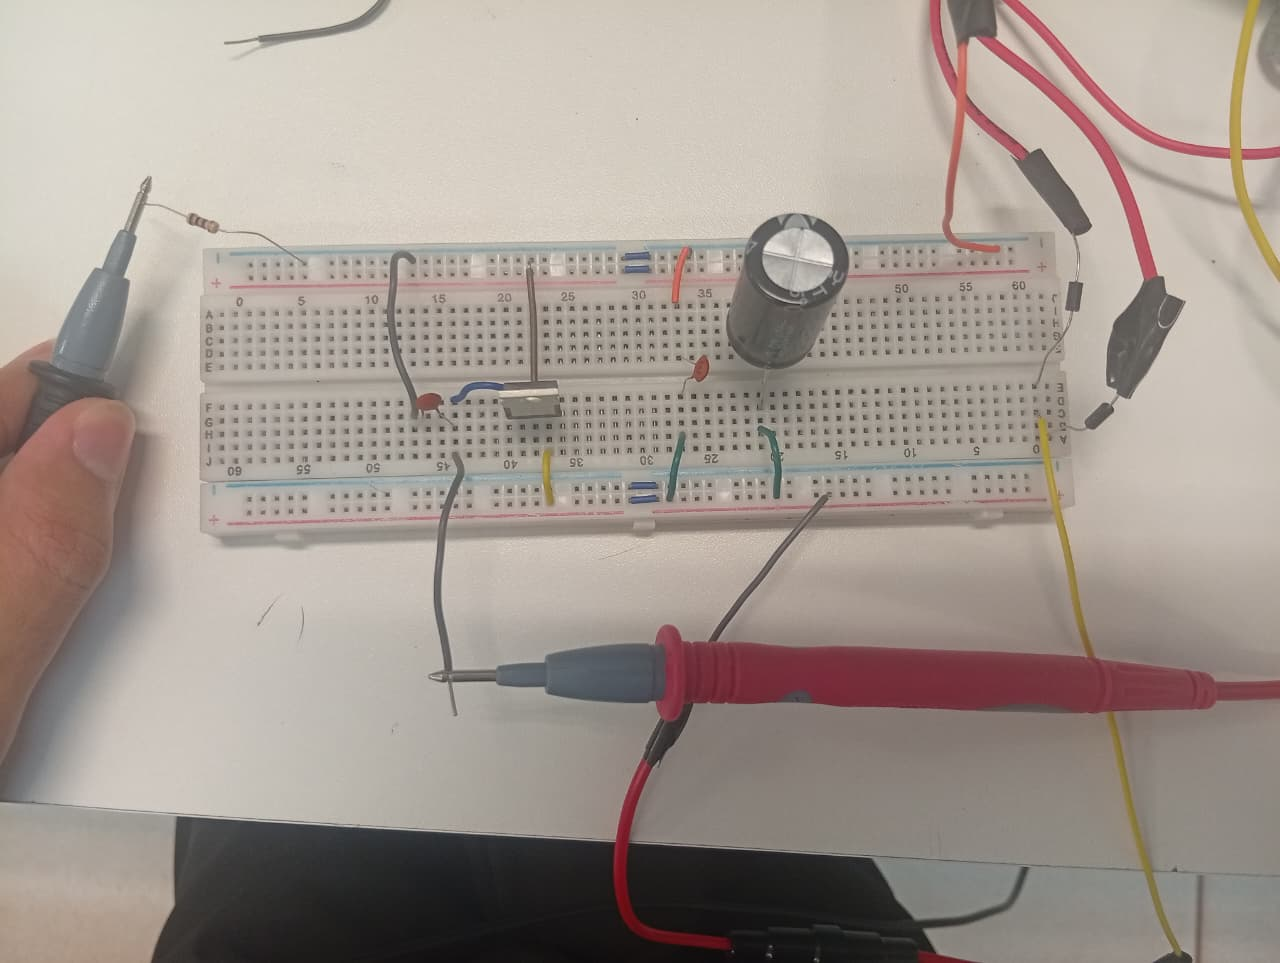
\includegraphics[width=\columnwidth,height=5.6cm,keepaspectratio]{Images/exp6_protoboard-multimetro_com-resistencia-100-ohm-corrente.jpeg}
\caption{Experimento 6 --- Montagem com o multímetro em série entre o pino~3 do LM7812 e o resistor de $100\,\Omega$ ao GND.}
\label{fig:exp6-proto}
\end{figure}

\begin{figure}[H]
\centering
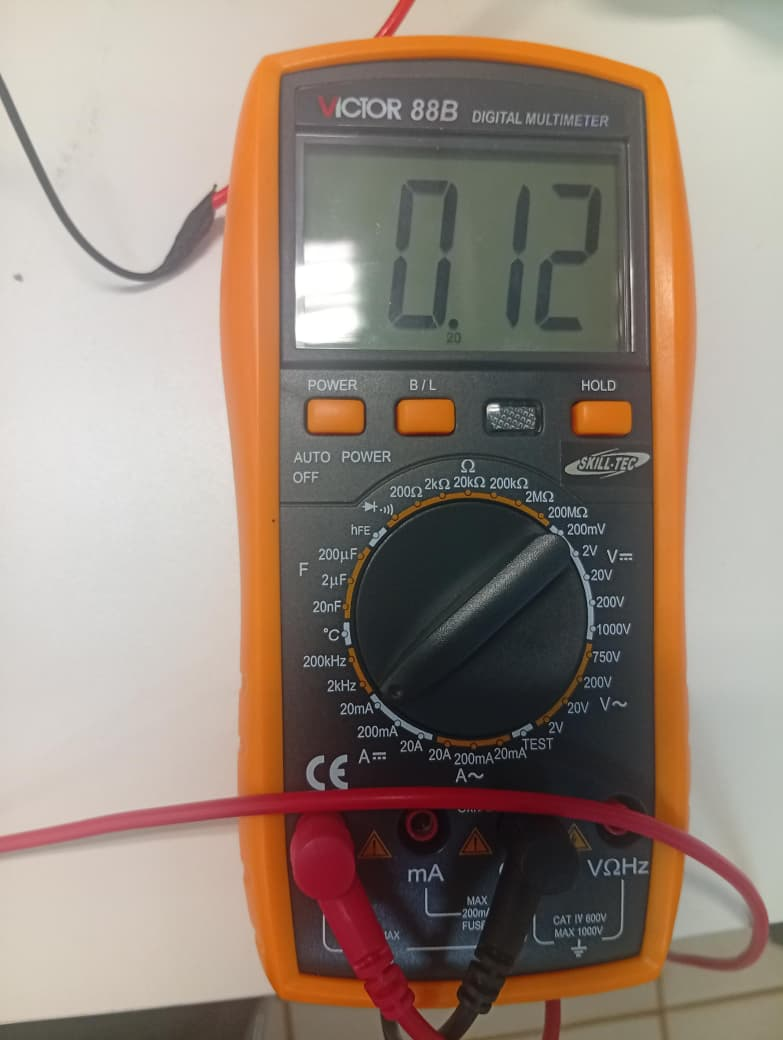
\includegraphics[width=\columnwidth,height=5.6cm,keepaspectratio]{Images/exp6_multimetro_com-resistencia-100-ohm-corrente.jpeg}
\caption{Experimento 6 --- Multímetro Victor 88B com ponta vermelha no borne $20\,\text{A}$, indicando $0{,}12\,\text{A}$ ($120\,\text{mA}$) DC sobre a carga de $100\,\Omega$. A posição do seletor na fotografia não coincide com o borne utilizado.}
\label{fig:exp6-corrente}
\end{figure}

\textbf{Valor medido.} O visor (Figura~\ref{fig:exp6-corrente}) indica $0{,}12\,\text{A}$, com resolução de $0{,}01\,\text{A}$. A posição do seletor na fotografia não coincide com o borne de $20\,\text{A}$ utilizado; a leitura é registrada como indicada.

\textbf{Esperado e desvio.} Com $V_o = 11{,}95\,\text{V}$ (medido com LED + $1\,\text{k}\Omega$):
\begin{equation}
I_{\text{teór}} = \frac{V_o}{R} = \frac{11{,}95\,\text{V}}{100\,\Omega} = 0{,}1195\,\text{A} = 119{,}5\,\text{mA}.
\label{eq:ohm}
\end{equation}
Com a tolerância de $\pm 5\%$ do resistor, a faixa esperada é $11{,}95/105 \approx 113{,}8\,\text{mA}$ a $11{,}95/95 \approx 125{,}8\,\text{mA}$. A leitura de $0{,}12\,\text{A}$ (desvio de $+0{,}4\%$ em relação a $119{,}5\,\text{mA}$), com resolução de $0{,}01\,\text{A}$, é compatível com essa faixa. A queda de tensão do amperímetro e o valor real do resistor não foram avaliados.

\textbf{Potência no resistor.} A potência dissipada é $P = V_o I = 11{,}95 \times 0{,}1195 \approx 1{,}43\,\text{W}$. Um resistor de $1/4\,\text{W}$ ficaria sobrecarregado ($\approx 5{,}7$ vezes sua potência nominal). A potência nominal do resistor utilizado não foi registrada. Recomenda-se resistor de potência nominal $\geq 2\,\text{W}$ para esse ensaio.

\subsection{Verificação Teórica a $1\,\text{A}$ (Análise Teórica, Não Ensaiada)}
\label{sec:teoria1A}

Esta subseção é uma análise teórica, não ensaiada: a fonte foi validada experimentalmente até $0{,}12\,\text{A}$ e projetada e analisada para $1\,\text{A}$. As premissas são: secundário de $12\,\text{V}$ RMS a $1\,\text{A}$ (especificação do trabalho; a tensão sob carga não foi medida), $V_D = 0{,}7\,\text{V}$, $f_{\text{ret}} = 120\,\text{Hz}$, $C = 4700\,\mu\text{F}$ e entrada mínima do regulador de $12\,\text{V} + 2\,\text{V} = 14\,\text{V}$ (\textit{dropout} de \textit{datasheet}~\cite{ds_lm7812}).

\textbf{Rede nominal.}
\begin{equation}
V_{p,\text{ret}} = 12\sqrt{2} - 0{,}7 \approx 16{,}27\,\text{V},
\label{eq:teoria_nom}
\end{equation}
\begin{equation}
\Delta V_r = \frac{1\,\text{A}}{120 \times 4700\,\mu\text{F}} \approx 1{,}77\,\text{V}_{\text{pp}},
\label{eq:teoria_ripple}
\end{equation}
\begin{equation}
V_{\text{vale}} = 16{,}27 - 1{,}77 \approx 14{,}5\,\text{V}.
\label{eq:teoria_vale}
\end{equation}
Em relação ao mínimo de $\approx 14\,\text{V}$, a margem é de $\approx 0{,}5\,\text{V}$.

\textbf{Rede $-10\%$.} Com $0{,}9 \times 12\,\text{V}$:
\begin{equation}
V_{p,\text{ret}} = 0{,}9 \times 12\sqrt{2} - 0{,}7 \approx 14{,}57\,\text{V},
\label{eq:teoria_rede}
\end{equation}
\begin{equation}
V_{\text{vale}} = 14{,}57 - 1{,}77 \approx 12{,}8\,\text{V}.
\end{equation}
Como $12{,}8\,\text{V} < 14\,\text{V}$, o regulador sai de regulação nos vales e o \textit{ripple} aparece na saída.

\textbf{Dissipação no regulador.} A tensão média na entrada é $V_{\text{méd}} \approx 16{,}27 - 1{,}77/2 \approx 15{,}4\,\text{V}$, e
\begin{equation}
P_D \approx (15{,}4 - 12) \times 1\,\text{A} \approx 3{,}4\,\text{W}.
\label{eq:teoria_pd}
\end{equation}
O valor de $6{,}0\,\text{W}$, obtido com a tensão sem carga, $(17{,}96 - 11{,}95) \times 1\,\text{A}$, é apenas um limite superior.

\textbf{Análise térmica.} Adota-se $T_a = 30\,^\circ\mathrm{C}$ (hipótese, não verificada). Como o componente utilizado possui gravação comercial SCE7812, sem folha de dados própria publicada pelo fabricante ou distribuidor, adotam-se os parâmetros térmicos do \href{https://www.ti.com/lit/ds/symlink/lm340.pdf}{Datasheet do LM7812}. Conforme os valores clássicos apresentados na seção 6.1 do documento, utilizam-se $R_{\theta JA} = 54\,^\circ\mathrm{C/W}$ e $R_{\theta JC} = 4\,^\circ\mathrm{C/W}$, além de $T_{j,\max} = 150\,^\circ\mathrm{C}$ (máximo absoluto, com operação recomendada até $125\,^\circ\mathrm{C}$). Sem dissipador,

\begin{equation}
\Delta T = P_D R_{\theta JA} \approx 3{,}4\,\mathrm{W} \times 54\,^\circ\mathrm{C/W} = 183{,}6\,^\circ\mathrm{C},
\tag{19}
\end{equation}

\begin{equation}
T_j = T_a + \Delta T = 30 + 183{,}6 = 213{,}6\,^\circ\mathrm{C},
\tag{20}
\end{equation}

e verifica-se que $T_j > T_{j,\max}$, indicando que a operação sem dissipador não é termicamente adequada. O dissipador necessário deve satisfazer

\begin{equation}
R_{\theta SA} \leq \frac{T_{j,\max} - T_a}{P_D} - R_{\theta JC} - R_{\theta CS},
\tag{21}
\end{equation}

com $R_{\theta CS}$ representando a resistência térmica da interface caixa--dissipador. Como não foi utilizado dissipador, esse parâmetro não se aplica à montagem realizada. O dissipador não consta na Tabela I, pois não foi adquirido.

\subsection{Síntese dos Resultados Experimentais}

A Tabela~\ref{tab:resumo} consolida os valores esperados ou calculados e as grandezas medidas.

\begin{table*}[t]
\renewcommand{\tablename}{TABELA}
\caption{Resumo comparativo entre valores esperados/calculados e medições.}
\label{tab:resumo}
\centering
\scriptsize
\setlength{\tabcolsep}{4pt}
\begin{tabular}{lp{2.4cm}p{3.1cm}p{3.3cm}p{1.5cm}p{4.9cm}}
\hline
Exp. & Condição & Esperado/calculado & Medido & Desvio (\%) & Observação \\
\hline
1 & Secundário em vazio (osciloscópio) & $60\,\text{Hz}$; $V_{\text{RMS}}$ nominal $12\,\text{V}$ & $60{,}01\,\text{Hz}$ (contador); $V_{p} = 19{,}1\,\text{V}$ (exibido $V_{\text{pp}} = 382\,\text{V}$, fator $1/10$); $V_{\text{RMS}} \approx 13{,}5\,\text{V}$ & $+0{,}01$ (freq.); $+12{,}5$ ($V_{\text{RMS}}$) & Atenuação $10\times$ (fator $1/10$) validada; $59{,}8\,\text{Hz}$ no osciloscópio ($-0{,}33\%$). \\
1 & Secundário em vazio (multímetro) & $V_{\text{RMS}} \approx 13{,}5\,\text{V}$ (osciloscópio), função V$\sim$ & $0{,}00\,\text{V}$ (função DC) & -- & Falha de procedimento; não é resultado do ensaio. \\
2A & Pós-diodos, $1\,\text{k}\Omega$, sem filtro & $V_{\text{DC}} = 12{,}16\,\text{V}$ ($V_p = 19{,}1\,\text{V}$); $11{,}71\,\text{V}$ ($18{,}4\,\text{V}$) & $\text{Mean} = 11{,}9\,\text{V}$; $120{,}08\,\text{Hz}$ (contador) & $-2{,}1$; $+1{,}6$ & Concordância dentro de $\approx \pm 2\%$; fator $1\times$; $V_{\text{pp}} = 19{,}1\,\text{V}$, $T = 8{,}36\,\text{ms}$. \\
2B & Com $4700\,\mu\text{F}$ & Nível DC próximo ao pico ($18{,}4\,\text{V}$) & $17{,}9\,\text{V}$ (exibido $179\,\text{V}$, fator $1/10$); $17{,}96\,\text{V}$ (multímetro, Exp.~3) & $-2{,}7$ & Resultado válido: nível DC. Janela de $240\,\mu\text{s}$ não mostra o \textit{ripple}. \\
3A & Pino 1, DC & $\geq 14\,\text{V}$ ($12\,\text{V}$ + \textit{dropout}) & $17{,}96\,\text{V}$ & -- & Validado; margem $\approx 4\,\text{V}$ sobre $14\,\text{V}$ e $\approx 6\,\text{V}$ sobre $12\,\text{V}$. \\
3B/C & \textit{Ripple} no pino 1, sem $\to$ com LED & $8{,}9 \to 24{,}8\,\text{mV}_{\text{pp}}$ & $\approx 1{,}3 \to 3{,}0\,\text{mV}_{\text{pp}}$ (exibidos) & $-85$; $-88$ & Amplitude absoluta não validada (fator da ponta não registrado); crescimento de $2{,}3\times$ contra $2{,}8\times$ previsto. \\
4 & Pino 3 com LED + $1\,\text{k}\Omega$, DC & $12{,}00\,\text{V}$ ($11{,}5$ a $12{,}5\,\text{V}$) & $11{,}95\,\text{V}$ & $-0{,}42$ & Dentro de $\pm 4\%$. \\
4 & \textit{Ripple} no pino 3 & Muito menor que na entrada & $\lesssim 0{,}6\,\text{mV}_{\text{pp}}$ (limite de leitura) & -- & Redução $\approx 14$ a $16\,\text{dB}$, apenas limite inferior; $55$ a $70\,\text{dB}$ são de \textit{datasheet}, não medidos. \\
5 & Sem $\times$ com LED + $1\,\text{k}\Omega$ & Sem variação detectável ($<$ incerteza de $\pm 0{,}08\,\text{V}$) & $11{,}93\,\text{V}$ e $11{,}95\,\text{V}$ & $-0{,}17$ (regulação de carga) & Leituras indistinguíveis; $\Delta I \approx 9\,\text{mA}$ não exercita a regulação. \\
6 & Carga de $100\,\Omega$, amperímetro em série & $119{,}5\,\text{mA}$ ($113{,}8$ a $125{,}8\,\text{mA}$) & $0{,}12\,\text{A}$ & $+0{,}4$ & Compatível; resolução de $0{,}01\,\text{A}$; $P = 1{,}43\,\text{W}$ no resistor. \\
\hline
\end{tabular}
\end{table*}

